\documentclass{article}

% Course report in the NeurIPS 2026 format. "preprint" shows the author names and removes line numbers.
\PassOptionsToPackage{numbers,sort&compress}{natbib}
\usepackage[preprint]{neurips_2026}

\usepackage[utf8]{inputenc}
\usepackage[T1]{fontenc}
\usepackage{lmodern}
\usepackage{float}  % [H] keeps each appendix table and figure under its own heading; loaded before hyperref
\usepackage{hyperref}
\usepackage{url}
\usepackage{booktabs}
\usepackage{amsmath}
\usepackage{amsfonts}
\usepackage{nicefrac}
\usepackage{microtype}
\usepackage{xcolor}
\usepackage{graphicx}

% generated by make_assets.py -- do not edit
\makeatletter
\newcommand{\num}[1]{\@ifundefined{num@#1}{\textbf{??}}{\csname num@#1\endcsname}}
\makeatother
\expandafter\def\csname num@acc@cnn@aug@clean\endcsname{53.5}
\expandafter\def\csname num@acc@cnn@aug@n0.025\endcsname{52.9}
\expandafter\def\csname num@acc@cnn@aug@n0.05\endcsname{51.8}
\expandafter\def\csname num@acc@cnn@aug@n0.1\endcsname{48.2}
\expandafter\def\csname num@acc@cnn@aug@n0.15\endcsname{44.4}
\expandafter\def\csname num@acc@cnn@aug@n0.2\endcsname{40.1}
\expandafter\def\csname num@acc@cnn@aug@n0.3\endcsname{33.3}
\expandafter\def\csname num@acc@cnn@aug@n0.4\endcsname{28.6}
\expandafter\def\csname num@acc@cnn@aug@n0.5\endcsname{26.9}
\expandafter\def\csname num@acc@cnn@aug@navg\endcsname{47.5}
\expandafter\def\csname num@acc@cnn@aug@r16\endcsname{35.9}
\expandafter\def\csname num@acc@cnn@aug@r24\endcsname{41.2}
\expandafter\def\csname num@acc@cnn@aug@r32\endcsname{47.1}
\expandafter\def\csname num@acc@cnn@aug@r4\endcsname{16.3}
\expandafter\def\csname num@acc@cnn@aug@r40\endcsname{49.7}
\expandafter\def\csname num@acc@cnn@aug@r8\endcsname{23.0}
\expandafter\def\csname num@acc@cnn@aug@ravg\endcsname{39.4}
\expandafter\def\csname num@acc@cnn@ref@clean\endcsname{53.9}
\expandafter\def\csname num@acc@cnn@ref@n0.025\endcsname{51.7}
\expandafter\def\csname num@acc@cnn@ref@n0.05\endcsname{45.4}
\expandafter\def\csname num@acc@cnn@ref@n0.1\endcsname{31.2}
\expandafter\def\csname num@acc@cnn@ref@n0.15\endcsname{23.2}
\expandafter\def\csname num@acc@cnn@ref@n0.2\endcsname{20.4}
\expandafter\def\csname num@acc@cnn@ref@n0.3\endcsname{18.6}
\expandafter\def\csname num@acc@cnn@ref@n0.4\endcsname{17.8}
\expandafter\def\csname num@acc@cnn@ref@n0.5\endcsname{17.7}
\expandafter\def\csname num@acc@cnn@ref@navg\endcsname{34.4}
\expandafter\def\csname num@acc@cnn@ref@r16\endcsname{35.0}
\expandafter\def\csname num@acc@cnn@ref@r24\endcsname{39.3}
\expandafter\def\csname num@acc@cnn@ref@r32\endcsname{45.8}
\expandafter\def\csname num@acc@cnn@ref@r4\endcsname{15.9}
\expandafter\def\csname num@acc@cnn@ref@r40\endcsname{49.7}
\expandafter\def\csname num@acc@cnn@ref@r8\endcsname{23.7}
\expandafter\def\csname num@acc@cnn@ref@ravg\endcsname{38.7}
\expandafter\def\csname num@acc@cnn@std@clean\endcsname{53.2}
\expandafter\def\csname num@acc@cnn@std@n0.025\endcsname{51.3}
\expandafter\def\csname num@acc@cnn@std@n0.05\endcsname{47.1}
\expandafter\def\csname num@acc@cnn@std@n0.1\endcsname{36.1}
\expandafter\def\csname num@acc@cnn@std@n0.15\endcsname{28.3}
\expandafter\def\csname num@acc@cnn@std@n0.2\endcsname{24.9}
\expandafter\def\csname num@acc@cnn@std@n0.3\endcsname{23.5}
\expandafter\def\csname num@acc@cnn@std@n0.4\endcsname{22.5}
\expandafter\def\csname num@acc@cnn@std@n0.5\endcsname{22.1}
\expandafter\def\csname num@acc@cnn@std@navg\endcsname{37.5}
\expandafter\def\csname num@acc@cnn@std@r16\endcsname{34.4}
\expandafter\def\csname num@acc@cnn@std@r24\endcsname{38.8}
\expandafter\def\csname num@acc@cnn@std@r32\endcsname{45.0}
\expandafter\def\csname num@acc@cnn@std@r4\endcsname{14.7}
\expandafter\def\csname num@acc@cnn@std@r40\endcsname{48.4}
\expandafter\def\csname num@acc@cnn@std@r8\endcsname{23.5}
\expandafter\def\csname num@acc@cnn@std@ravg\endcsname{38.0}
\expandafter\def\csname num@acc@resnet18@aug@clean\endcsname{63.1}
\expandafter\def\csname num@acc@resnet18@aug@n0.025\endcsname{62.2}
\expandafter\def\csname num@acc@resnet18@aug@n0.05\endcsname{60.8}
\expandafter\def\csname num@acc@resnet18@aug@n0.1\endcsname{58.1}
\expandafter\def\csname num@acc@resnet18@aug@n0.15\endcsname{53.5}
\expandafter\def\csname num@acc@resnet18@aug@n0.2\endcsname{49.0}
\expandafter\def\csname num@acc@resnet18@aug@n0.3\endcsname{40.4}
\expandafter\def\csname num@acc@resnet18@aug@n0.4\endcsname{33.3}
\expandafter\def\csname num@acc@resnet18@aug@n0.5\endcsname{27.6}
\expandafter\def\csname num@acc@resnet18@aug@navg\endcsname{56.7}
\expandafter\def\csname num@acc@resnet18@aug@r16\endcsname{43.5}
\expandafter\def\csname num@acc@resnet18@aug@r24\endcsname{52.0}
\expandafter\def\csname num@acc@resnet18@aug@r32\endcsname{57.3}
\expandafter\def\csname num@acc@resnet18@aug@r4\endcsname{23.7}
\expandafter\def\csname num@acc@resnet18@aug@r40\endcsname{60.3}
\expandafter\def\csname num@acc@resnet18@aug@r8\endcsname{25.5}
\expandafter\def\csname num@acc@resnet18@aug@ravg\endcsname{47.7}
\expandafter\def\csname num@acc@resnet18@ref@clean\endcsname{63.7}
\expandafter\def\csname num@acc@resnet18@ref@n0.025\endcsname{56.2}
\expandafter\def\csname num@acc@resnet18@ref@n0.05\endcsname{44.8}
\expandafter\def\csname num@acc@resnet18@ref@n0.1\endcsname{27.1}
\expandafter\def\csname num@acc@resnet18@ref@n0.15\endcsname{21.1}
\expandafter\def\csname num@acc@resnet18@ref@n0.2\endcsname{19.2}
\expandafter\def\csname num@acc@resnet18@ref@n0.3\endcsname{17.7}
\expandafter\def\csname num@acc@resnet18@ref@n0.4\endcsname{17.1}
\expandafter\def\csname num@acc@resnet18@ref@n0.5\endcsname{16.4}
\expandafter\def\csname num@acc@resnet18@ref@navg\endcsname{33.7}
\expandafter\def\csname num@acc@resnet18@ref@r16\endcsname{29.5}
\expandafter\def\csname num@acc@resnet18@ref@r24\endcsname{42.1}
\expandafter\def\csname num@acc@resnet18@ref@r32\endcsname{51.6}
\expandafter\def\csname num@acc@resnet18@ref@r4\endcsname{20.0}
\expandafter\def\csname num@acc@resnet18@ref@r40\endcsname{56.2}
\expandafter\def\csname num@acc@resnet18@ref@r8\endcsname{19.1}
\expandafter\def\csname num@acc@resnet18@ref@ravg\endcsname{39.7}
\expandafter\def\csname num@acc@resnet18@std@clean\endcsname{61.2}
\expandafter\def\csname num@acc@resnet18@std@n0.025\endcsname{55.3}
\expandafter\def\csname num@acc@resnet18@std@n0.05\endcsname{46.2}
\expandafter\def\csname num@acc@resnet18@std@n0.1\endcsname{33.1}
\expandafter\def\csname num@acc@resnet18@std@n0.15\endcsname{28.4}
\expandafter\def\csname num@acc@resnet18@std@n0.2\endcsname{26.1}
\expandafter\def\csname num@acc@resnet18@std@n0.3\endcsname{23.4}
\expandafter\def\csname num@acc@resnet18@std@n0.4\endcsname{22.9}
\expandafter\def\csname num@acc@resnet18@std@n0.5\endcsname{21.8}
\expandafter\def\csname num@acc@resnet18@std@navg\endcsname{37.8}
\expandafter\def\csname num@acc@resnet18@std@r16\endcsname{30.1}
\expandafter\def\csname num@acc@resnet18@std@r24\endcsname{39.2}
\expandafter\def\csname num@acc@resnet18@std@r32\endcsname{48.4}
\expandafter\def\csname num@acc@resnet18@std@r4\endcsname{19.1}
\expandafter\def\csname num@acc@resnet18@std@r40\endcsname{54.3}
\expandafter\def\csname num@acc@resnet18@std@r8\endcsname{20.7}
\expandafter\def\csname num@acc@resnet18@std@ravg\endcsname{38.6}
\expandafter\def\csname num@acc@vit_b16@aug@clean\endcsname{68.5}
\expandafter\def\csname num@acc@vit_b16@aug@n0.025\endcsname{68.0}
\expandafter\def\csname num@acc@vit_b16@aug@n0.05\endcsname{66.8}
\expandafter\def\csname num@acc@vit_b16@aug@n0.1\endcsname{62.3}
\expandafter\def\csname num@acc@vit_b16@aug@n0.15\endcsname{58.6}
\expandafter\def\csname num@acc@vit_b16@aug@n0.2\endcsname{53.5}
\expandafter\def\csname num@acc@vit_b16@aug@n0.3\endcsname{45.2}
\expandafter\def\csname num@acc@vit_b16@aug@n0.4\endcsname{38.9}
\expandafter\def\csname num@acc@vit_b16@aug@n0.5\endcsname{34.0}
\expandafter\def\csname num@acc@vit_b16@aug@navg\endcsname{61.9}
\expandafter\def\csname num@acc@vit_b16@aug@r16\endcsname{47.7}
\expandafter\def\csname num@acc@vit_b16@aug@r24\endcsname{55.2}
\expandafter\def\csname num@acc@vit_b16@aug@r32\endcsname{61.9}
\expandafter\def\csname num@acc@vit_b16@aug@r4\endcsname{17.5}
\expandafter\def\csname num@acc@vit_b16@aug@r40\endcsname{64.8}
\expandafter\def\csname num@acc@vit_b16@aug@r8\endcsname{19.2}
\expandafter\def\csname num@acc@vit_b16@aug@ravg\endcsname{49.8}
\expandafter\def\csname num@acc@vit_b16@ref@clean\endcsname{69.5}
\expandafter\def\csname num@acc@vit_b16@ref@n0.025\endcsname{65.3}
\expandafter\def\csname num@acc@vit_b16@ref@n0.05\endcsname{57.5}
\expandafter\def\csname num@acc@vit_b16@ref@n0.1\endcsname{40.3}
\expandafter\def\csname num@acc@vit_b16@ref@n0.15\endcsname{30.2}
\expandafter\def\csname num@acc@vit_b16@ref@n0.2\endcsname{22.8}
\expandafter\def\csname num@acc@vit_b16@ref@n0.3\endcsname{17.2}
\expandafter\def\csname num@acc@vit_b16@ref@n0.4\endcsname{16.2}
\expandafter\def\csname num@acc@vit_b16@ref@n0.5\endcsname{15.7}
\expandafter\def\csname num@acc@vit_b16@ref@navg\endcsname{43.2}
\expandafter\def\csname num@acc@vit_b16@ref@r16\endcsname{38.6}
\expandafter\def\csname num@acc@vit_b16@ref@r24\endcsname{49.1}
\expandafter\def\csname num@acc@vit_b16@ref@r32\endcsname{59.3}
\expandafter\def\csname num@acc@vit_b16@ref@r4\endcsname{16.8}
\expandafter\def\csname num@acc@vit_b16@ref@r40\endcsname{63.7}
\expandafter\def\csname num@acc@vit_b16@ref@r8\endcsname{17.5}
\expandafter\def\csname num@acc@vit_b16@ref@ravg\endcsname{45.7}
\expandafter\def\csname num@acc@vit_b16@std@clean\endcsname{69.3}
\expandafter\def\csname num@acc@vit_b16@std@n0.025\endcsname{65.2}
\expandafter\def\csname num@acc@vit_b16@std@n0.05\endcsname{58.5}
\expandafter\def\csname num@acc@vit_b16@std@n0.1\endcsname{42.1}
\expandafter\def\csname num@acc@vit_b16@std@n0.15\endcsname{31.1}
\expandafter\def\csname num@acc@vit_b16@std@n0.2\endcsname{23.0}
\expandafter\def\csname num@acc@vit_b16@std@n0.3\endcsname{18.2}
\expandafter\def\csname num@acc@vit_b16@std@n0.4\endcsname{16.6}
\expandafter\def\csname num@acc@vit_b16@std@n0.5\endcsname{15.7}
\expandafter\def\csname num@acc@vit_b16@std@navg\endcsname{44.0}
\expandafter\def\csname num@acc@vit_b16@std@r16\endcsname{39.8}
\expandafter\def\csname num@acc@vit_b16@std@r24\endcsname{49.5}
\expandafter\def\csname num@acc@vit_b16@std@r32\endcsname{59.0}
\expandafter\def\csname num@acc@vit_b16@std@r4\endcsname{17.2}
\expandafter\def\csname num@acc@vit_b16@std@r40\endcsname{63.3}
\expandafter\def\csname num@acc@vit_b16@std@r8\endcsname{17.6}
\expandafter\def\csname num@acc@vit_b16@std@ravg\endcsname{45.8}
\expandafter\def\csname num@accsd@cnn@aug@clean\endcsname{0.4}
\expandafter\def\csname num@accsd@cnn@aug@navg\endcsname{0.5}
\expandafter\def\csname num@accsd@cnn@aug@ravg\endcsname{0.3}
\expandafter\def\csname num@accsd@cnn@ref@clean\endcsname{0.5}
\expandafter\def\csname num@accsd@cnn@ref@navg\endcsname{3.6}
\expandafter\def\csname num@accsd@cnn@ref@ravg\endcsname{2.1}
\expandafter\def\csname num@accsd@cnn@std@clean\endcsname{1.3}
\expandafter\def\csname num@accsd@cnn@std@navg\endcsname{0.4}
\expandafter\def\csname num@accsd@cnn@std@ravg\endcsname{0.4}
\expandafter\def\csname num@accsd@resnet18@aug@clean\endcsname{1.1}
\expandafter\def\csname num@accsd@resnet18@aug@navg\endcsname{0.4}
\expandafter\def\csname num@accsd@resnet18@aug@ravg\endcsname{2.3}
\expandafter\def\csname num@accsd@resnet18@ref@clean\endcsname{0.3}
\expandafter\def\csname num@accsd@resnet18@ref@navg\endcsname{2.8}
\expandafter\def\csname num@accsd@resnet18@ref@ravg\endcsname{1.2}
\expandafter\def\csname num@accsd@resnet18@std@clean\endcsname{1.4}
\expandafter\def\csname num@accsd@resnet18@std@navg\endcsname{2.5}
\expandafter\def\csname num@accsd@resnet18@std@ravg\endcsname{0.9}
\expandafter\def\csname num@accsd@vit_b16@aug@clean\endcsname{0.5}
\expandafter\def\csname num@accsd@vit_b16@aug@navg\endcsname{0.1}
\expandafter\def\csname num@accsd@vit_b16@aug@ravg\endcsname{0.7}
\expandafter\def\csname num@accsd@vit_b16@ref@clean\endcsname{0.4}
\expandafter\def\csname num@accsd@vit_b16@ref@navg\endcsname{0.3}
\expandafter\def\csname num@accsd@vit_b16@ref@ravg\endcsname{0.4}
\expandafter\def\csname num@accsd@vit_b16@std@clean\endcsname{1.1}
\expandafter\def\csname num@accsd@vit_b16@std@navg\endcsname{0.3}
\expandafter\def\csname num@accsd@vit_b16@std@ravg\endcsname{0.9}
\expandafter\def\csname num@archdiff@resnet18@cnn@aug@clean\endcsname{9.6}
\expandafter\def\csname num@archdiff@resnet18@cnn@aug@navg\endcsname{9.2}
\expandafter\def\csname num@archdiff@resnet18@cnn@aug@ravg\endcsname{8.3}
\expandafter\def\csname num@archdiff@resnet18@cnn@ref@clean\endcsname{9.8}
\expandafter\def\csname num@archdiff@resnet18@cnn@ref@navg\endcsname{$-$0.7}
\expandafter\def\csname num@archdiff@resnet18@cnn@ref@ravg\endcsname{1.0}
\expandafter\def\csname num@archdiff@resnet18@cnn@std@clean\endcsname{8.1}
\expandafter\def\csname num@archdiff@resnet18@cnn@std@navg\endcsname{0.3}
\expandafter\def\csname num@archdiff@resnet18@cnn@std@ravg\endcsname{0.6}
\expandafter\def\csname num@archdiff@vit_b16@cnn@aug@clean\endcsname{15.1}
\expandafter\def\csname num@archdiff@vit_b16@cnn@aug@navg\endcsname{14.4}
\expandafter\def\csname num@archdiff@vit_b16@cnn@aug@ravg\endcsname{10.4}
\expandafter\def\csname num@archdiff@vit_b16@cnn@ref@clean\endcsname{15.5}
\expandafter\def\csname num@archdiff@vit_b16@cnn@ref@navg\endcsname{8.8}
\expandafter\def\csname num@archdiff@vit_b16@cnn@ref@ravg\endcsname{7.0}
\expandafter\def\csname num@archdiff@vit_b16@cnn@std@clean\endcsname{16.1}
\expandafter\def\csname num@archdiff@vit_b16@cnn@std@navg\endcsname{6.5}
\expandafter\def\csname num@archdiff@vit_b16@cnn@std@ravg\endcsname{7.8}
\expandafter\def\csname num@archdiff@vit_b16@resnet18@aug@clean\endcsname{5.5}
\expandafter\def\csname num@archdiff@vit_b16@resnet18@aug@navg\endcsname{5.1}
\expandafter\def\csname num@archdiff@vit_b16@resnet18@aug@ravg\endcsname{2.1}
\expandafter\def\csname num@archdiff@vit_b16@resnet18@ref@clean\endcsname{5.7}
\expandafter\def\csname num@archdiff@vit_b16@resnet18@ref@navg\endcsname{9.5}
\expandafter\def\csname num@archdiff@vit_b16@resnet18@ref@ravg\endcsname{6.0}
\expandafter\def\csname num@archdiff@vit_b16@resnet18@std@clean\endcsname{8.0}
\expandafter\def\csname num@archdiff@vit_b16@resnet18@std@navg\endcsname{6.2}
\expandafter\def\csname num@archdiff@vit_b16@resnet18@std@ravg\endcsname{7.3}
\expandafter\def\csname num@audit@conflicting_label_groups\endcsname{57}
\expandafter\def\csname num@audit@cross_split_duplicate_groups\endcsname{557}
\expandafter\def\csname num@audit@duplicate_groups\endcsname{1{,}516}
\expandafter\def\csname num@audit@n_rows\endcsname{35{,}887}
\expandafter\def\csname num@audit@n_unique_images\endcsname{34{,}034}
\expandafter\def\csname num@audit@rows_removed_conflicting\endcsname{160}
\expandafter\def\csname num@audit@rows_removed_redundant\endcsname{1{,}750}
\expandafter\def\csname num@augp@cnn\endcsname{0.5}
\expandafter\def\csname num@augp@resnet18\endcsname{0.8}
\expandafter\def\csname num@augp@vit_b16\endcsname{0.8}
\expandafter\def\csname num@augref@cnn@clean\endcsname{$-$0.5}
\expandafter\def\csname num@augref@cnn@navg\endcsname{+13.1}
\expandafter\def\csname num@augref@cnn@ravg\endcsname{+0.7}
\expandafter\def\csname num@augref@resnet18@clean\endcsname{$-$0.7}
\expandafter\def\csname num@augref@resnet18@navg\endcsname{+23.1}
\expandafter\def\csname num@augref@resnet18@ravg\endcsname{+8.0}
\expandafter\def\csname num@augref@vit_b16@clean\endcsname{$-$0.9}
\expandafter\def\csname num@augref@vit_b16@navg\endcsname{+18.6}
\expandafter\def\csname num@augref@vit_b16@ravg\endcsname{+4.1}
\expandafter\def\csname num@augrefabs@cnn@clean\endcsname{0.5}
\expandafter\def\csname num@augrefabs@cnn@navg\endcsname{13.1}
\expandafter\def\csname num@augrefabs@cnn@ravg\endcsname{0.7}
\expandafter\def\csname num@augrefabs@resnet18@clean\endcsname{0.7}
\expandafter\def\csname num@augrefabs@resnet18@navg\endcsname{23.1}
\expandafter\def\csname num@augrefabs@resnet18@ravg\endcsname{8.0}
\expandafter\def\csname num@augrefabs@vit_b16@clean\endcsname{0.9}
\expandafter\def\csname num@augrefabs@vit_b16@navg\endcsname{18.6}
\expandafter\def\csname num@augrefabs@vit_b16@ravg\endcsname{4.1}
\expandafter\def\csname num@augsigma@cnn\endcsname{0.2}
\expandafter\def\csname num@augsigma@resnet18\endcsname{0.2}
\expandafter\def\csname num@augsigma@vit_b16\endcsname{0.2}
\expandafter\def\csname num@below@cnn@aug@noise\endcsname{0.15}
\expandafter\def\csname num@below@cnn@aug@res\endcsname{32}
\expandafter\def\csname num@below@cnn@ref@noise\endcsname{0.05}
\expandafter\def\csname num@below@cnn@ref@res\endcsname{32}
\expandafter\def\csname num@below@cnn@std@noise\endcsname{0.05}
\expandafter\def\csname num@below@cnn@std@res\endcsname{32}
\expandafter\def\csname num@below@resnet18@aug@noise\endcsname{0.15}
\expandafter\def\csname num@below@resnet18@aug@res\endcsname{24}
\expandafter\def\csname num@below@resnet18@ref@noise\endcsname{0.025}
\expandafter\def\csname num@below@resnet18@ref@res\endcsname{40}
\expandafter\def\csname num@below@resnet18@std@noise\endcsname{0.05}
\expandafter\def\csname num@below@resnet18@std@res\endcsname{40}
\expandafter\def\csname num@below@vit_b16@aug@noise\endcsname{0.15}
\expandafter\def\csname num@below@vit_b16@aug@res\endcsname{24}
\expandafter\def\csname num@below@vit_b16@ref@noise\endcsname{0.05}
\expandafter\def\csname num@below@vit_b16@ref@res\endcsname{32}
\expandafter\def\csname num@below@vit_b16@std@noise\endcsname{0.05}
\expandafter\def\csname num@below@vit_b16@std@res\endcsname{32}
\expandafter\def\csname num@delta@cnn@clean\endcsname{+0.3}
\expandafter\def\csname num@delta@cnn@n0.025\endcsname{+1.7}
\expandafter\def\csname num@delta@cnn@n0.05\endcsname{+4.7}
\expandafter\def\csname num@delta@cnn@n0.1\endcsname{+12.1}
\expandafter\def\csname num@delta@cnn@n0.15\endcsname{+16.2}
\expandafter\def\csname num@delta@cnn@n0.2\endcsname{+15.2}
\expandafter\def\csname num@delta@cnn@navg\endcsname{+10.0}
\expandafter\def\csname num@delta@cnn@r16\endcsname{+1.5}
\expandafter\def\csname num@delta@cnn@r24\endcsname{+2.4}
\expandafter\def\csname num@delta@cnn@r32\endcsname{+2.1}
\expandafter\def\csname num@delta@cnn@r40\endcsname{+1.3}
\expandafter\def\csname num@delta@cnn@r8\endcsname{$-$0.5}
\expandafter\def\csname num@delta@cnn@ravg\endcsname{+1.4}
\expandafter\def\csname num@delta@resnet18@clean\endcsname{+1.8}
\expandafter\def\csname num@delta@resnet18@n0.025\endcsname{+6.9}
\expandafter\def\csname num@delta@resnet18@n0.05\endcsname{+14.7}
\expandafter\def\csname num@delta@resnet18@n0.1\endcsname{+25.0}
\expandafter\def\csname num@delta@resnet18@n0.15\endcsname{+25.1}
\expandafter\def\csname num@delta@resnet18@n0.2\endcsname{+22.9}
\expandafter\def\csname num@delta@resnet18@navg\endcsname{+18.9}
\expandafter\def\csname num@delta@resnet18@r16\endcsname{+13.4}
\expandafter\def\csname num@delta@resnet18@r24\endcsname{+12.7}
\expandafter\def\csname num@delta@resnet18@r32\endcsname{+8.9}
\expandafter\def\csname num@delta@resnet18@r40\endcsname{+6.0}
\expandafter\def\csname num@delta@resnet18@r8\endcsname{+4.8}
\expandafter\def\csname num@delta@resnet18@ravg\endcsname{+9.2}
\expandafter\def\csname num@delta@vit_b16@clean\endcsname{$-$0.7}
\expandafter\def\csname num@delta@vit_b16@n0.025\endcsname{+2.8}
\expandafter\def\csname num@delta@vit_b16@n0.05\endcsname{+8.4}
\expandafter\def\csname num@delta@vit_b16@n0.1\endcsname{+20.2}
\expandafter\def\csname num@delta@vit_b16@n0.15\endcsname{+27.6}
\expandafter\def\csname num@delta@vit_b16@n0.2\endcsname{+30.5}
\expandafter\def\csname num@delta@vit_b16@navg\endcsname{+17.9}
\expandafter\def\csname num@delta@vit_b16@r16\endcsname{+7.9}
\expandafter\def\csname num@delta@vit_b16@r24\endcsname{+5.7}
\expandafter\def\csname num@delta@vit_b16@r32\endcsname{+3.0}
\expandafter\def\csname num@delta@vit_b16@r40\endcsname{+1.4}
\expandafter\def\csname num@delta@vit_b16@r8\endcsname{+1.6}
\expandafter\def\csname num@delta@vit_b16@ravg\endcsname{+3.9}
\expandafter\def\csname num@deltasd@cnn@clean\endcsname{1.4}
\expandafter\def\csname num@deltasd@cnn@navg\endcsname{0.9}
\expandafter\def\csname num@deltasd@cnn@ravg\endcsname{0.3}
\expandafter\def\csname num@deltasd@resnet18@clean\endcsname{2.3}
\expandafter\def\csname num@deltasd@resnet18@navg\endcsname{2.4}
\expandafter\def\csname num@deltasd@resnet18@ravg\endcsname{1.4}
\expandafter\def\csname num@deltasd@vit_b16@clean\endcsname{0.8}
\expandafter\def\csname num@deltasd@vit_b16@navg\endcsname{0.3}
\expandafter\def\csname num@deltasd@vit_b16@ravg\endcsname{1.5}
\expandafter\def\csname num@epochs@cnn@aug\endcsname{49, 43, 51}
\expandafter\def\csname num@epochs@cnn@ref\endcsname{32, 60, 58}
\expandafter\def\csname num@epochs@cnn@std\endcsname{28, 22, 32}
\expandafter\def\csname num@epochs@resnet18@aug\endcsname{4, 3, 5}
\expandafter\def\csname num@epochs@resnet18@ref\endcsname{6, 2, 4}
\expandafter\def\csname num@epochs@resnet18@std\endcsname{6, 1, 1}
\expandafter\def\csname num@epochs@vit_b16@aug\endcsname{4, 4, 4}
\expandafter\def\csname num@epochs@vit_b16@ref\endcsname{4, 3, 4}
\expandafter\def\csname num@epochs@vit_b16@std\endcsname{3, 2, 4}
\expandafter\def\csname num@gpuhours@final\endcsname{3.7}
\expandafter\def\csname num@gpuhours@protocol\endcsname{2.5}
\expandafter\def\csname num@gpuhours@ref\endcsname{1.2}
\expandafter\def\csname num@haslrcheck\endcsname{1}
\expandafter\def\csname num@lr@cnn\endcsname{$1{\times}10^{-3}$}
\expandafter\def\csname num@lr@resnet18\endcsname{$3{\times}10^{-4}$}
\expandafter\def\csname num@lr@vit_b16\endcsname{$5{\times}10^{-5}$}
\expandafter\def\csname num@lrcheck@resnet18@absdiff\endcsname{0.007}
\expandafter\def\csname num@lrcheck@resnet18@clean\endcsname{60.7}
\expandafter\def\csname num@lrcheck@resnet18@diff\endcsname{$-$0.007}
\expandafter\def\csname num@lrcheck@resnet18@epoch\endcsname{3}
\expandafter\def\csname num@lrcheck@resnet18@lr\endcsname{$1{\times}10^{-3}$}
\expandafter\def\csname num@lrcheck@resnet18@noisy\endcsname{36.1}
\expandafter\def\csname num@lrcheck@resnet18@score\endcsname{0.484}
\expandafter\def\csname num@lrcheck@resnet18@selscore\endcsname{0.491}
\expandafter\def\csname num@lrcheck@vit_b16@absdiff\endcsname{0.004}
\expandafter\def\csname num@lrcheck@vit_b16@clean\endcsname{68.7}
\expandafter\def\csname num@lrcheck@vit_b16@diff\endcsname{+0.004}
\expandafter\def\csname num@lrcheck@vit_b16@epoch\endcsname{3}
\expandafter\def\csname num@lrcheck@vit_b16@lr\endcsname{$1{\times}10^{-4}$}
\expandafter\def\csname num@lrcheck@vit_b16@noisy\endcsname{43.2}
\expandafter\def\csname num@lrcheck@vit_b16@score\endcsname{0.560}
\expandafter\def\csname num@lrcheck@vit_b16@selscore\endcsname{0.556}
\expandafter\def\csname num@macro_f1@cnn@aug@clean\endcsname{45.9}
\expandafter\def\csname num@macro_f1@cnn@aug@n0.025\endcsname{45.3}
\expandafter\def\csname num@macro_f1@cnn@aug@n0.05\endcsname{44.3}
\expandafter\def\csname num@macro_f1@cnn@aug@n0.1\endcsname{40.1}
\expandafter\def\csname num@macro_f1@cnn@aug@n0.15\endcsname{36.4}
\expandafter\def\csname num@macro_f1@cnn@aug@n0.2\endcsname{31.0}
\expandafter\def\csname num@macro_f1@cnn@aug@n0.3\endcsname{24.8}
\expandafter\def\csname num@macro_f1@cnn@aug@n0.4\endcsname{20.2}
\expandafter\def\csname num@macro_f1@cnn@aug@n0.5\endcsname{17.5}
\expandafter\def\csname num@macro_f1@cnn@aug@navg\endcsname{39.4}
\expandafter\def\csname num@macro_f1@cnn@aug@r16\endcsname{26.6}
\expandafter\def\csname num@macro_f1@cnn@aug@r24\endcsname{32.1}
\expandafter\def\csname num@macro_f1@cnn@aug@r32\endcsname{39.3}
\expandafter\def\csname num@macro_f1@cnn@aug@r4\endcsname{10.1}
\expandafter\def\csname num@macro_f1@cnn@aug@r40\endcsname{41.6}
\expandafter\def\csname num@macro_f1@cnn@aug@r8\endcsname{16.5}
\expandafter\def\csname num@macro_f1@cnn@aug@ravg\endcsname{31.2}
\expandafter\def\csname num@macro_f1@cnn@ref@clean\endcsname{46.1}
\expandafter\def\csname num@macro_f1@cnn@ref@n0.025\endcsname{44.7}
\expandafter\def\csname num@macro_f1@cnn@ref@n0.05\endcsname{38.4}
\expandafter\def\csname num@macro_f1@cnn@ref@n0.1\endcsname{23.8}
\expandafter\def\csname num@macro_f1@cnn@ref@n0.15\endcsname{14.5}
\expandafter\def\csname num@macro_f1@cnn@ref@n0.2\endcsname{10.9}
\expandafter\def\csname num@macro_f1@cnn@ref@n0.3\endcsname{8.0}
\expandafter\def\csname num@macro_f1@cnn@ref@n0.4\endcsname{6.9}
\expandafter\def\csname num@macro_f1@cnn@ref@n0.5\endcsname{6.4}
\expandafter\def\csname num@macro_f1@cnn@ref@navg\endcsname{26.5}
\expandafter\def\csname num@macro_f1@cnn@ref@r16\endcsname{24.3}
\expandafter\def\csname num@macro_f1@cnn@ref@r24\endcsname{29.3}
\expandafter\def\csname num@macro_f1@cnn@ref@r32\endcsname{37.1}
\expandafter\def\csname num@macro_f1@cnn@ref@r4\endcsname{10.0}
\expandafter\def\csname num@macro_f1@cnn@ref@r40\endcsname{41.8}
\expandafter\def\csname num@macro_f1@cnn@ref@r8\endcsname{15.3}
\expandafter\def\csname num@macro_f1@cnn@ref@ravg\endcsname{29.6}
\expandafter\def\csname num@macro_f1@cnn@std@clean\endcsname{45.6}
\expandafter\def\csname num@macro_f1@cnn@std@n0.025\endcsname{43.9}
\expandafter\def\csname num@macro_f1@cnn@std@n0.05\endcsname{39.8}
\expandafter\def\csname num@macro_f1@cnn@std@n0.1\endcsname{28.3}
\expandafter\def\csname num@macro_f1@cnn@std@n0.15\endcsname{18.5}
\expandafter\def\csname num@macro_f1@cnn@std@n0.2\endcsname{13.5}
\expandafter\def\csname num@macro_f1@cnn@std@n0.3\endcsname{10.6}
\expandafter\def\csname num@macro_f1@cnn@std@n0.4\endcsname{9.2}
\expandafter\def\csname num@macro_f1@cnn@std@n0.5\endcsname{8.8}
\expandafter\def\csname num@macro_f1@cnn@std@navg\endcsname{28.8}
\expandafter\def\csname num@macro_f1@cnn@std@r16\endcsname{23.4}
\expandafter\def\csname num@macro_f1@cnn@std@r24\endcsname{28.1}
\expandafter\def\csname num@macro_f1@cnn@std@r32\endcsname{36.0}
\expandafter\def\csname num@macro_f1@cnn@std@r4\endcsname{10.6}
\expandafter\def\csname num@macro_f1@cnn@std@r40\endcsname{39.9}
\expandafter\def\csname num@macro_f1@cnn@std@r8\endcsname{15.5}
\expandafter\def\csname num@macro_f1@cnn@std@ravg\endcsname{28.6}
\expandafter\def\csname num@macro_f1@resnet18@aug@clean\endcsname{57.8}
\expandafter\def\csname num@macro_f1@resnet18@aug@n0.025\endcsname{56.1}
\expandafter\def\csname num@macro_f1@resnet18@aug@n0.05\endcsname{55.0}
\expandafter\def\csname num@macro_f1@resnet18@aug@n0.1\endcsname{52.4}
\expandafter\def\csname num@macro_f1@resnet18@aug@n0.15\endcsname{46.5}
\expandafter\def\csname num@macro_f1@resnet18@aug@n0.2\endcsname{42.7}
\expandafter\def\csname num@macro_f1@resnet18@aug@n0.3\endcsname{34.1}
\expandafter\def\csname num@macro_f1@resnet18@aug@n0.4\endcsname{27.9}
\expandafter\def\csname num@macro_f1@resnet18@aug@n0.5\endcsname{21.8}
\expandafter\def\csname num@macro_f1@resnet18@aug@navg\endcsname{50.5}
\expandafter\def\csname num@macro_f1@resnet18@aug@r16\endcsname{34.1}
\expandafter\def\csname num@macro_f1@resnet18@aug@r24\endcsname{44.4}
\expandafter\def\csname num@macro_f1@resnet18@aug@r32\endcsname{51.3}
\expandafter\def\csname num@macro_f1@resnet18@aug@r4\endcsname{7.7}
\expandafter\def\csname num@macro_f1@resnet18@aug@r40\endcsname{54.7}
\expandafter\def\csname num@macro_f1@resnet18@aug@r8\endcsname{12.3}
\expandafter\def\csname num@macro_f1@resnet18@aug@ravg\endcsname{39.3}
\expandafter\def\csname num@macro_f1@resnet18@ref@clean\endcsname{58.9}
\expandafter\def\csname num@macro_f1@resnet18@ref@n0.025\endcsname{48.5}
\expandafter\def\csname num@macro_f1@resnet18@ref@n0.05\endcsname{36.8}
\expandafter\def\csname num@macro_f1@resnet18@ref@n0.1\endcsname{15.6}
\expandafter\def\csname num@macro_f1@resnet18@ref@n0.15\endcsname{8.4}
\expandafter\def\csname num@macro_f1@resnet18@ref@n0.2\endcsname{6.5}
\expandafter\def\csname num@macro_f1@resnet18@ref@n0.3\endcsname{5.1}
\expandafter\def\csname num@macro_f1@resnet18@ref@n0.4\endcsname{5.3}
\expandafter\def\csname num@macro_f1@resnet18@ref@n0.5\endcsname{5.5}
\expandafter\def\csname num@macro_f1@resnet18@ref@navg\endcsname{23.2}
\expandafter\def\csname num@macro_f1@resnet18@ref@r16\endcsname{20.0}
\expandafter\def\csname num@macro_f1@resnet18@ref@r24\endcsname{30.6}
\expandafter\def\csname num@macro_f1@resnet18@ref@r32\endcsname{43.5}
\expandafter\def\csname num@macro_f1@resnet18@ref@r4\endcsname{7.5}
\expandafter\def\csname num@macro_f1@resnet18@ref@r40\endcsname{51.0}
\expandafter\def\csname num@macro_f1@resnet18@ref@r8\endcsname{7.6}
\expandafter\def\csname num@macro_f1@resnet18@ref@ravg\endcsname{30.5}
\expandafter\def\csname num@macro_f1@resnet18@std@clean\endcsname{53.4}
\expandafter\def\csname num@macro_f1@resnet18@std@n0.025\endcsname{46.3}
\expandafter\def\csname num@macro_f1@resnet18@std@n0.05\endcsname{34.9}
\expandafter\def\csname num@macro_f1@resnet18@std@n0.1\endcsname{20.2}
\expandafter\def\csname num@macro_f1@resnet18@std@n0.15\endcsname{13.9}
\expandafter\def\csname num@macro_f1@resnet18@std@n0.2\endcsname{11.2}
\expandafter\def\csname num@macro_f1@resnet18@std@n0.3\endcsname{8.3}
\expandafter\def\csname num@macro_f1@resnet18@std@n0.4\endcsname{7.6}
\expandafter\def\csname num@macro_f1@resnet18@std@n0.5\endcsname{7.4}
\expandafter\def\csname num@macro_f1@resnet18@std@navg\endcsname{25.3}
\expandafter\def\csname num@macro_f1@resnet18@std@r16\endcsname{18.1}
\expandafter\def\csname num@macro_f1@resnet18@std@r24\endcsname{26.7}
\expandafter\def\csname num@macro_f1@resnet18@std@r32\endcsname{38.1}
\expandafter\def\csname num@macro_f1@resnet18@std@r4\endcsname{7.4}
\expandafter\def\csname num@macro_f1@resnet18@std@r40\endcsname{45.1}
\expandafter\def\csname num@macro_f1@resnet18@std@r8\endcsname{8.4}
\expandafter\def\csname num@macro_f1@resnet18@std@ravg\endcsname{27.3}
\expandafter\def\csname num@macro_f1@vit_b16@aug@clean\endcsname{63.9}
\expandafter\def\csname num@macro_f1@vit_b16@aug@n0.025\endcsname{63.6}
\expandafter\def\csname num@macro_f1@vit_b16@aug@n0.05\endcsname{62.8}
\expandafter\def\csname num@macro_f1@vit_b16@aug@n0.1\endcsname{56.7}
\expandafter\def\csname num@macro_f1@vit_b16@aug@n0.15\endcsname{52.8}
\expandafter\def\csname num@macro_f1@vit_b16@aug@n0.2\endcsname{45.6}
\expandafter\def\csname num@macro_f1@vit_b16@aug@n0.3\endcsname{37.3}
\expandafter\def\csname num@macro_f1@vit_b16@aug@n0.4\endcsname{30.7}
\expandafter\def\csname num@macro_f1@vit_b16@aug@n0.5\endcsname{26.0}
\expandafter\def\csname num@macro_f1@vit_b16@aug@navg\endcsname{56.3}
\expandafter\def\csname num@macro_f1@vit_b16@aug@r16\endcsname{40.0}
\expandafter\def\csname num@macro_f1@vit_b16@aug@r24\endcsname{48.9}
\expandafter\def\csname num@macro_f1@vit_b16@aug@r32\endcsname{56.7}
\expandafter\def\csname num@macro_f1@vit_b16@aug@r4\endcsname{6.0}
\expandafter\def\csname num@macro_f1@vit_b16@aug@r40\endcsname{60.2}
\expandafter\def\csname num@macro_f1@vit_b16@aug@r8\endcsname{10.0}
\expandafter\def\csname num@macro_f1@vit_b16@aug@ravg\endcsname{43.2}
\expandafter\def\csname num@macro_f1@vit_b16@ref@clean\endcsname{65.8}
\expandafter\def\csname num@macro_f1@vit_b16@ref@n0.025\endcsname{59.6}
\expandafter\def\csname num@macro_f1@vit_b16@ref@n0.05\endcsname{50.4}
\expandafter\def\csname num@macro_f1@vit_b16@ref@n0.1\endcsname{34.5}
\expandafter\def\csname num@macro_f1@vit_b16@ref@n0.15\endcsname{25.0}
\expandafter\def\csname num@macro_f1@vit_b16@ref@n0.2\endcsname{17.4}
\expandafter\def\csname num@macro_f1@vit_b16@ref@n0.3\endcsname{10.4}
\expandafter\def\csname num@macro_f1@vit_b16@ref@n0.4\endcsname{8.9}
\expandafter\def\csname num@macro_f1@vit_b16@ref@n0.5\endcsname{8.0}
\expandafter\def\csname num@macro_f1@vit_b16@ref@navg\endcsname{37.4}
\expandafter\def\csname num@macro_f1@vit_b16@ref@r16\endcsname{32.3}
\expandafter\def\csname num@macro_f1@vit_b16@ref@r24\endcsname{41.1}
\expandafter\def\csname num@macro_f1@vit_b16@ref@r32\endcsname{54.9}
\expandafter\def\csname num@macro_f1@vit_b16@ref@r4\endcsname{7.1}
\expandafter\def\csname num@macro_f1@vit_b16@ref@r40\endcsname{59.5}
\expandafter\def\csname num@macro_f1@vit_b16@ref@r8\endcsname{11.6}
\expandafter\def\csname num@macro_f1@vit_b16@ref@ravg\endcsname{39.9}
\expandafter\def\csname num@macro_f1@vit_b16@std@clean\endcsname{65.3}
\expandafter\def\csname num@macro_f1@vit_b16@std@n0.025\endcsname{59.7}
\expandafter\def\csname num@macro_f1@vit_b16@std@n0.05\endcsname{50.7}
\expandafter\def\csname num@macro_f1@vit_b16@std@n0.1\endcsname{35.6}
\expandafter\def\csname num@macro_f1@vit_b16@std@n0.15\endcsname{25.6}
\expandafter\def\csname num@macro_f1@vit_b16@std@n0.2\endcsname{17.5}
\expandafter\def\csname num@macro_f1@vit_b16@std@n0.3\endcsname{11.5}
\expandafter\def\csname num@macro_f1@vit_b16@std@n0.4\endcsname{9.2}
\expandafter\def\csname num@macro_f1@vit_b16@std@n0.5\endcsname{8.0}
\expandafter\def\csname num@macro_f1@vit_b16@std@navg\endcsname{37.8}
\expandafter\def\csname num@macro_f1@vit_b16@std@r16\endcsname{32.8}
\expandafter\def\csname num@macro_f1@vit_b16@std@r24\endcsname{42.5}
\expandafter\def\csname num@macro_f1@vit_b16@std@r32\endcsname{53.9}
\expandafter\def\csname num@macro_f1@vit_b16@std@r4\endcsname{7.4}
\expandafter\def\csname num@macro_f1@vit_b16@std@r40\endcsname{59.6}
\expandafter\def\csname num@macro_f1@vit_b16@std@r8\endcsname{10.8}
\expandafter\def\csname num@macro_f1@vit_b16@std@ravg\endcsname{39.9}
\expandafter\def\csname num@macro_f1sd@cnn@aug@clean\endcsname{1.1}
\expandafter\def\csname num@macro_f1sd@cnn@aug@navg\endcsname{0.5}
\expandafter\def\csname num@macro_f1sd@cnn@aug@ravg\endcsname{0.3}
\expandafter\def\csname num@macro_f1sd@cnn@ref@clean\endcsname{1.6}
\expandafter\def\csname num@macro_f1sd@cnn@ref@navg\endcsname{2.8}
\expandafter\def\csname num@macro_f1sd@cnn@ref@ravg\endcsname{3.2}
\expandafter\def\csname num@macro_f1sd@cnn@std@clean\endcsname{2.4}
\expandafter\def\csname num@macro_f1sd@cnn@std@navg\endcsname{2.1}
\expandafter\def\csname num@macro_f1sd@cnn@std@ravg\endcsname{1.7}
\expandafter\def\csname num@macro_f1sd@resnet18@aug@clean\endcsname{1.1}
\expandafter\def\csname num@macro_f1sd@resnet18@aug@navg\endcsname{1.0}
\expandafter\def\csname num@macro_f1sd@resnet18@aug@ravg\endcsname{2.1}
\expandafter\def\csname num@macro_f1sd@resnet18@ref@clean\endcsname{0.8}
\expandafter\def\csname num@macro_f1sd@resnet18@ref@navg\endcsname{3.2}
\expandafter\def\csname num@macro_f1sd@resnet18@ref@ravg\endcsname{0.8}
\expandafter\def\csname num@macro_f1sd@resnet18@std@clean\endcsname{5.1}
\expandafter\def\csname num@macro_f1sd@resnet18@std@navg\endcsname{2.8}
\expandafter\def\csname num@macro_f1sd@resnet18@std@ravg\endcsname{1.5}
\expandafter\def\csname num@macro_f1sd@vit_b16@aug@clean\endcsname{0.5}
\expandafter\def\csname num@macro_f1sd@vit_b16@aug@navg\endcsname{0.7}
\expandafter\def\csname num@macro_f1sd@vit_b16@aug@ravg\endcsname{0.4}
\expandafter\def\csname num@macro_f1sd@vit_b16@ref@clean\endcsname{0.5}
\expandafter\def\csname num@macro_f1sd@vit_b16@ref@navg\endcsname{1.0}
\expandafter\def\csname num@macro_f1sd@vit_b16@ref@ravg\endcsname{0.7}
\expandafter\def\csname num@macro_f1sd@vit_b16@std@clean\endcsname{2.0}
\expandafter\def\csname num@macro_f1sd@vit_b16@std@navg\endcsname{0.6}
\expandafter\def\csname num@macro_f1sd@vit_b16@std@ravg\endcsname{0.9}
\expandafter\def\csname num@majority\endcsname{25.9}
\expandafter\def\csname num@nfinal\endcsname{18}
\expandafter\def\csname num@nref\endcsname{9}
\expandafter\def\csname num@nseeds@cnn@aug\endcsname{3}
\expandafter\def\csname num@nseeds@cnn@ref\endcsname{3}
\expandafter\def\csname num@nseeds@cnn@std\endcsname{3}
\expandafter\def\csname num@nseeds@resnet18@aug\endcsname{3}
\expandafter\def\csname num@nseeds@resnet18@ref\endcsname{3}
\expandafter\def\csname num@nseeds@resnet18@std\endcsname{3}
\expandafter\def\csname num@nseeds@vit_b16@aug\endcsname{3}
\expandafter\def\csname num@nseeds@vit_b16@ref\endcsname{3}
\expandafter\def\csname num@nseeds@vit_b16@std\endcsname{3}
\expandafter\def\csname num@ntest\endcsname{3{,}268}
\expandafter\def\csname num@params@cnn\endcsname{93{,}575}
\expandafter\def\csname num@params@resnet18\endcsname{11{,}180{,}103}
\expandafter\def\csname num@params@vit_b16\endcsname{85{,}804{,}039}
\expandafter\def\csname num@recall@cnn@aug@angry@clean\endcsname{34}
\expandafter\def\csname num@recall@cnn@aug@angry@n0.1\endcsname{30}
\expandafter\def\csname num@recall@cnn@aug@angry@r24\endcsname{12}
\expandafter\def\csname num@recall@cnn@aug@disgust@clean\endcsname{10}
\expandafter\def\csname num@recall@cnn@aug@disgust@n0.1\endcsname{5}
\expandafter\def\csname num@recall@cnn@aug@disgust@r24\endcsname{4}
\expandafter\def\csname num@recall@cnn@aug@fear@clean\endcsname{30}
\expandafter\def\csname num@recall@cnn@aug@fear@n0.1\endcsname{23}
\expandafter\def\csname num@recall@cnn@aug@fear@r24\endcsname{23}
\expandafter\def\csname num@recall@cnn@aug@happy@clean\endcsname{78}
\expandafter\def\csname num@recall@cnn@aug@happy@n0.1\endcsname{74}
\expandafter\def\csname num@recall@cnn@aug@happy@r24\endcsname{68}
\expandafter\def\csname num@recall@cnn@aug@neutral@clean\endcsname{56}
\expandafter\def\csname num@recall@cnn@aug@neutral@n0.1\endcsname{50}
\expandafter\def\csname num@recall@cnn@aug@neutral@r24\endcsname{28}
\expandafter\def\csname num@recall@cnn@aug@sad@clean\endcsname{50}
\expandafter\def\csname num@recall@cnn@aug@sad@n0.1\endcsname{45}
\expandafter\def\csname num@recall@cnn@aug@sad@r24\endcsname{63}
\expandafter\def\csname num@recall@cnn@aug@surprise@clean\endcsname{59}
\expandafter\def\csname num@recall@cnn@aug@surprise@n0.1\endcsname{52}
\expandafter\def\csname num@recall@cnn@aug@surprise@r24\endcsname{27}
\expandafter\def\csname num@recall@cnn@ref@angry@clean\endcsname{43}
\expandafter\def\csname num@recall@cnn@ref@angry@n0.1\endcsname{21}
\expandafter\def\csname num@recall@cnn@ref@angry@r24\endcsname{18}
\expandafter\def\csname num@recall@cnn@ref@disgust@clean\endcsname{10}
\expandafter\def\csname num@recall@cnn@ref@disgust@n0.1\endcsname{4}
\expandafter\def\csname num@recall@cnn@ref@disgust@r24\endcsname{1}
\expandafter\def\csname num@recall@cnn@ref@fear@clean\endcsname{29}
\expandafter\def\csname num@recall@cnn@ref@fear@n0.1\endcsname{7}
\expandafter\def\csname num@recall@cnn@ref@fear@r24\endcsname{18}
\expandafter\def\csname num@recall@cnn@ref@happy@clean\endcsname{80}
\expandafter\def\csname num@recall@cnn@ref@happy@n0.1\endcsname{34}
\expandafter\def\csname num@recall@cnn@ref@happy@r24\endcsname{71}
\expandafter\def\csname num@recall@cnn@ref@neutral@clean\endcsname{51}
\expandafter\def\csname num@recall@cnn@ref@neutral@n0.1\endcsname{69}
\expandafter\def\csname num@recall@cnn@ref@neutral@r24\endcsname{23}
\expandafter\def\csname num@recall@cnn@ref@sad@clean\endcsname{49}
\expandafter\def\csname num@recall@cnn@ref@sad@n0.1\endcsname{19}
\expandafter\def\csname num@recall@cnn@ref@sad@r24\endcsname{54}
\expandafter\def\csname num@recall@cnn@ref@surprise@clean\endcsname{58}
\expandafter\def\csname num@recall@cnn@ref@surprise@n0.1\endcsname{29}
\expandafter\def\csname num@recall@cnn@ref@surprise@r24\endcsname{26}
\expandafter\def\csname num@recall@cnn@std@angry@clean\endcsname{41}
\expandafter\def\csname num@recall@cnn@std@angry@n0.1\endcsname{29}
\expandafter\def\csname num@recall@cnn@std@angry@r24\endcsname{15}
\expandafter\def\csname num@recall@cnn@std@disgust@clean\endcsname{11}
\expandafter\def\csname num@recall@cnn@std@disgust@n0.1\endcsname{1}
\expandafter\def\csname num@recall@cnn@std@disgust@r24\endcsname{1}
\expandafter\def\csname num@recall@cnn@std@fear@clean\endcsname{31}
\expandafter\def\csname num@recall@cnn@std@fear@n0.1\endcsname{8}
\expandafter\def\csname num@recall@cnn@std@fear@r24\endcsname{22}
\expandafter\def\csname num@recall@cnn@std@happy@clean\endcsname{82}
\expandafter\def\csname num@recall@cnn@std@happy@n0.1\endcsname{52}
\expandafter\def\csname num@recall@cnn@std@happy@r24\endcsname{76}
\expandafter\def\csname num@recall@cnn@std@neutral@clean\endcsname{49}
\expandafter\def\csname num@recall@cnn@std@neutral@n0.1\endcsname{59}
\expandafter\def\csname num@recall@cnn@std@neutral@r24\endcsname{20}
\expandafter\def\csname num@recall@cnn@std@sad@clean\endcsname{42}
\expandafter\def\csname num@recall@cnn@std@sad@n0.1\endcsname{20}
\expandafter\def\csname num@recall@cnn@std@sad@r24\endcsname{48}
\expandafter\def\csname num@recall@cnn@std@surprise@clean\endcsname{61}
\expandafter\def\csname num@recall@cnn@std@surprise@n0.1\endcsname{38}
\expandafter\def\csname num@recall@cnn@std@surprise@r24\endcsname{21}
\expandafter\def\csname num@recall@resnet18@aug@angry@clean\endcsname{51}
\expandafter\def\csname num@recall@resnet18@aug@angry@n0.1\endcsname{42}
\expandafter\def\csname num@recall@resnet18@aug@angry@r24\endcsname{22}
\expandafter\def\csname num@recall@resnet18@aug@disgust@clean\endcsname{30}
\expandafter\def\csname num@recall@resnet18@aug@disgust@n0.1\endcsname{24}
\expandafter\def\csname num@recall@resnet18@aug@disgust@r24\endcsname{17}
\expandafter\def\csname num@recall@resnet18@aug@fear@clean\endcsname{37}
\expandafter\def\csname num@recall@resnet18@aug@fear@n0.1\endcsname{30}
\expandafter\def\csname num@recall@resnet18@aug@fear@r24\endcsname{26}
\expandafter\def\csname num@recall@resnet18@aug@happy@clean\endcsname{87}
\expandafter\def\csname num@recall@resnet18@aug@happy@n0.1\endcsname{82}
\expandafter\def\csname num@recall@resnet18@aug@happy@r24\endcsname{79}
\expandafter\def\csname num@recall@resnet18@aug@neutral@clean\endcsname{69}
\expandafter\def\csname num@recall@resnet18@aug@neutral@n0.1\endcsname{67}
\expandafter\def\csname num@recall@resnet18@aug@neutral@r24\endcsname{53}
\expandafter\def\csname num@recall@resnet18@aug@sad@clean\endcsname{53}
\expandafter\def\csname num@recall@resnet18@aug@sad@n0.1\endcsname{48}
\expandafter\def\csname num@recall@resnet18@aug@sad@r24\endcsname{61}
\expandafter\def\csname num@recall@resnet18@aug@surprise@clean\endcsname{68}
\expandafter\def\csname num@recall@resnet18@aug@surprise@n0.1\endcsname{66}
\expandafter\def\csname num@recall@resnet18@aug@surprise@r24\endcsname{48}
\expandafter\def\csname num@recall@resnet18@ref@angry@clean\endcsname{62}
\expandafter\def\csname num@recall@resnet18@ref@angry@n0.1\endcsname{7}
\expandafter\def\csname num@recall@resnet18@ref@angry@r24\endcsname{28}
\expandafter\def\csname num@recall@resnet18@ref@disgust@clean\endcsname{40}
\expandafter\def\csname num@recall@resnet18@ref@disgust@n0.1\endcsname{0}
\expandafter\def\csname num@recall@resnet18@ref@disgust@r24\endcsname{2}
\expandafter\def\csname num@recall@resnet18@ref@fear@clean\endcsname{43}
\expandafter\def\csname num@recall@resnet18@ref@fear@n0.1\endcsname{5}
\expandafter\def\csname num@recall@resnet18@ref@fear@r24\endcsname{31}
\expandafter\def\csname num@recall@resnet18@ref@happy@clean\endcsname{88}
\expandafter\def\csname num@recall@resnet18@ref@happy@n0.1\endcsname{33}
\expandafter\def\csname num@recall@resnet18@ref@happy@r24\endcsname{83}
\expandafter\def\csname num@recall@resnet18@ref@neutral@clean\endcsname{67}
\expandafter\def\csname num@recall@resnet18@ref@neutral@n0.1\endcsname{6}
\expandafter\def\csname num@recall@resnet18@ref@neutral@r24\endcsname{20}
\expandafter\def\csname num@recall@resnet18@ref@sad@clean\endcsname{43}
\expandafter\def\csname num@recall@resnet18@ref@sad@n0.1\endcsname{87}
\expandafter\def\csname num@recall@resnet18@ref@sad@r24\endcsname{37}
\expandafter\def\csname num@recall@resnet18@ref@surprise@clean\endcsname{66}
\expandafter\def\csname num@recall@resnet18@ref@surprise@n0.1\endcsname{6}
\expandafter\def\csname num@recall@resnet18@ref@surprise@r24\endcsname{22}
\expandafter\def\csname num@recall@resnet18@std@angry@clean\endcsname{53}
\expandafter\def\csname num@recall@resnet18@std@angry@n0.1\endcsname{17}
\expandafter\def\csname num@recall@resnet18@std@angry@r24\endcsname{20}
\expandafter\def\csname num@recall@resnet18@std@disgust@clean\endcsname{18}
\expandafter\def\csname num@recall@resnet18@std@disgust@n0.1\endcsname{0}
\expandafter\def\csname num@recall@resnet18@std@disgust@r24\endcsname{4}
\expandafter\def\csname num@recall@resnet18@std@fear@clean\endcsname{40}
\expandafter\def\csname num@recall@resnet18@std@fear@n0.1\endcsname{3}
\expandafter\def\csname num@recall@resnet18@std@fear@r24\endcsname{12}
\expandafter\def\csname num@recall@resnet18@std@happy@clean\endcsname{91}
\expandafter\def\csname num@recall@resnet18@std@happy@n0.1\endcsname{68}
\expandafter\def\csname num@recall@resnet18@std@happy@r24\endcsname{88}
\expandafter\def\csname num@recall@resnet18@std@neutral@clean\endcsname{56}
\expandafter\def\csname num@recall@resnet18@std@neutral@n0.1\endcsname{23}
\expandafter\def\csname num@recall@resnet18@std@neutral@r24\endcsname{16}
\expandafter\def\csname num@recall@resnet18@std@sad@clean\endcsname{49}
\expandafter\def\csname num@recall@resnet18@std@sad@n0.1\endcsname{43}
\expandafter\def\csname num@recall@resnet18@std@sad@r24\endcsname{39}
\expandafter\def\csname num@recall@resnet18@std@surprise@clean\endcsname{65}
\expandafter\def\csname num@recall@resnet18@std@surprise@n0.1\endcsname{13}
\expandafter\def\csname num@recall@resnet18@std@surprise@r24\endcsname{24}
\expandafter\def\csname num@recall@vit_b16@aug@angry@clean\endcsname{60}
\expandafter\def\csname num@recall@vit_b16@aug@angry@n0.1\endcsname{53}
\expandafter\def\csname num@recall@vit_b16@aug@angry@r24\endcsname{50}
\expandafter\def\csname num@recall@vit_b16@aug@disgust@clean\endcsname{40}
\expandafter\def\csname num@recall@vit_b16@aug@disgust@n0.1\endcsname{28}
\expandafter\def\csname num@recall@vit_b16@aug@disgust@r24\endcsname{14}
\expandafter\def\csname num@recall@vit_b16@aug@fear@clean\endcsname{47}
\expandafter\def\csname num@recall@vit_b16@aug@fear@n0.1\endcsname{38}
\expandafter\def\csname num@recall@vit_b16@aug@fear@r24\endcsname{29}
\expandafter\def\csname num@recall@vit_b16@aug@happy@clean\endcsname{91}
\expandafter\def\csname num@recall@vit_b16@aug@happy@n0.1\endcsname{86}
\expandafter\def\csname num@recall@vit_b16@aug@happy@r24\endcsname{78}
\expandafter\def\csname num@recall@vit_b16@aug@neutral@clean\endcsname{71}
\expandafter\def\csname num@recall@vit_b16@aug@neutral@n0.1\endcsname{64}
\expandafter\def\csname num@recall@vit_b16@aug@neutral@r24\endcsname{32}
\expandafter\def\csname num@recall@vit_b16@aug@sad@clean\endcsname{57}
\expandafter\def\csname num@recall@vit_b16@aug@sad@n0.1\endcsname{51}
\expandafter\def\csname num@recall@vit_b16@aug@sad@r24\endcsname{74}
\expandafter\def\csname num@recall@vit_b16@aug@surprise@clean\endcsname{73}
\expandafter\def\csname num@recall@vit_b16@aug@surprise@n0.1\endcsname{71}
\expandafter\def\csname num@recall@vit_b16@aug@surprise@r24\endcsname{55}
\expandafter\def\csname num@recall@vit_b16@ref@angry@clean\endcsname{60}
\expandafter\def\csname num@recall@vit_b16@ref@angry@n0.1\endcsname{32}
\expandafter\def\csname num@recall@vit_b16@ref@angry@r24\endcsname{50}
\expandafter\def\csname num@recall@vit_b16@ref@disgust@clean\endcsname{51}
\expandafter\def\csname num@recall@vit_b16@ref@disgust@n0.1\endcsname{1}
\expandafter\def\csname num@recall@vit_b16@ref@disgust@r24\endcsname{4}
\expandafter\def\csname num@recall@vit_b16@ref@fear@clean\endcsname{50}
\expandafter\def\csname num@recall@vit_b16@ref@fear@n0.1\endcsname{26}
\expandafter\def\csname num@recall@vit_b16@ref@fear@r24\endcsname{31}
\expandafter\def\csname num@recall@vit_b16@ref@happy@clean\endcsname{91}
\expandafter\def\csname num@recall@vit_b16@ref@happy@n0.1\endcsname{46}
\expandafter\def\csname num@recall@vit_b16@ref@happy@r24\endcsname{71}
\expandafter\def\csname num@recall@vit_b16@ref@neutral@clean\endcsname{69}
\expandafter\def\csname num@recall@vit_b16@ref@neutral@n0.1\endcsname{31}
\expandafter\def\csname num@recall@vit_b16@ref@neutral@r24\endcsname{22}
\expandafter\def\csname num@recall@vit_b16@ref@sad@clean\endcsname{60}
\expandafter\def\csname num@recall@vit_b16@ref@sad@n0.1\endcsname{64}
\expandafter\def\csname num@recall@vit_b16@ref@sad@r24\endcsname{62}
\expandafter\def\csname num@recall@vit_b16@ref@surprise@clean\endcsname{76}
\expandafter\def\csname num@recall@vit_b16@ref@surprise@n0.1\endcsname{38}
\expandafter\def\csname num@recall@vit_b16@ref@surprise@r24\endcsname{49}
\expandafter\def\csname num@recall@vit_b16@std@angry@clean\endcsname{63}
\expandafter\def\csname num@recall@vit_b16@std@angry@n0.1\endcsname{35}
\expandafter\def\csname num@recall@vit_b16@std@angry@r24\endcsname{51}
\expandafter\def\csname num@recall@vit_b16@std@disgust@clean\endcsname{54}
\expandafter\def\csname num@recall@vit_b16@std@disgust@n0.1\endcsname{1}
\expandafter\def\csname num@recall@vit_b16@std@disgust@r24\endcsname{9}
\expandafter\def\csname num@recall@vit_b16@std@fear@clean\endcsname{48}
\expandafter\def\csname num@recall@vit_b16@std@fear@n0.1\endcsname{20}
\expandafter\def\csname num@recall@vit_b16@std@fear@r24\endcsname{28}
\expandafter\def\csname num@recall@vit_b16@std@happy@clean\endcsname{91}
\expandafter\def\csname num@recall@vit_b16@std@happy@n0.1\endcsname{50}
\expandafter\def\csname num@recall@vit_b16@std@happy@r24\endcsname{71}
\expandafter\def\csname num@recall@vit_b16@std@neutral@clean\endcsname{71}
\expandafter\def\csname num@recall@vit_b16@std@neutral@n0.1\endcsname{38}
\expandafter\def\csname num@recall@vit_b16@std@neutral@r24\endcsname{22}
\expandafter\def\csname num@recall@vit_b16@std@sad@clean\endcsname{56}
\expandafter\def\csname num@recall@vit_b16@std@sad@n0.1\endcsname{62}
\expandafter\def\csname num@recall@vit_b16@std@sad@r24\endcsname{66}
\expandafter\def\csname num@recall@vit_b16@std@surprise@clean\endcsname{77}
\expandafter\def\csname num@recall@vit_b16@std@surprise@n0.1\endcsname{40}
\expandafter\def\csname num@recall@vit_b16@std@surprise@r24\endcsname{53}
\expandafter\def\csname num@refabs@cnn@clean\endcsname{0.8}
\expandafter\def\csname num@refabs@cnn@navg\endcsname{3.1}
\expandafter\def\csname num@refabs@cnn@ravg\endcsname{0.7}
\expandafter\def\csname num@refabs@resnet18@clean\endcsname{2.5}
\expandafter\def\csname num@refabs@resnet18@navg\endcsname{4.1}
\expandafter\def\csname num@refabs@resnet18@ravg\endcsname{1.1}
\expandafter\def\csname num@refabs@vit_b16@clean\endcsname{0.2}
\expandafter\def\csname num@refabs@vit_b16@navg\endcsname{0.8}
\expandafter\def\csname num@refabs@vit_b16@ravg\endcsname{0.2}
\expandafter\def\csname num@refdelta@cnn@clean\endcsname{+0.8}
\expandafter\def\csname num@refdelta@cnn@navg\endcsname{$-$3.1}
\expandafter\def\csname num@refdelta@cnn@ravg\endcsname{+0.7}
\expandafter\def\csname num@refdelta@resnet18@clean\endcsname{+2.5}
\expandafter\def\csname num@refdelta@resnet18@navg\endcsname{$-$4.1}
\expandafter\def\csname num@refdelta@resnet18@ravg\endcsname{+1.1}
\expandafter\def\csname num@refdelta@vit_b16@clean\endcsname{+0.2}
\expandafter\def\csname num@refdelta@vit_b16@navg\endcsname{$-$0.8}
\expandafter\def\csname num@refdelta@vit_b16@ravg\endcsname{$-$0.2}
\expandafter\def\csname num@refdeltasd@cnn@clean\endcsname{1.0}
\expandafter\def\csname num@refdeltasd@cnn@navg\endcsname{3.8}
\expandafter\def\csname num@refdeltasd@cnn@ravg\endcsname{1.9}
\expandafter\def\csname num@refdeltasd@resnet18@clean\endcsname{1.6}
\expandafter\def\csname num@refdeltasd@resnet18@navg\endcsname{4.3}
\expandafter\def\csname num@refdeltasd@resnet18@ravg\endcsname{1.6}
\expandafter\def\csname num@refdeltasd@vit_b16@clean\endcsname{0.7}
\expandafter\def\csname num@refdeltasd@vit_b16@navg\endcsname{0.5}
\expandafter\def\csname num@refdeltasd@vit_b16@ravg\endcsname{0.6}
\expandafter\def\csname num@rel@cnn@aug@n0.025\endcsname{99}
\expandafter\def\csname num@rel@cnn@aug@n0.05\endcsname{97}
\expandafter\def\csname num@rel@cnn@aug@n0.1\endcsname{90}
\expandafter\def\csname num@rel@cnn@aug@n0.15\endcsname{83}
\expandafter\def\csname num@rel@cnn@aug@n0.2\endcsname{75}
\expandafter\def\csname num@rel@cnn@aug@n0.3\endcsname{62}
\expandafter\def\csname num@rel@cnn@aug@n0.4\endcsname{53}
\expandafter\def\csname num@rel@cnn@aug@n0.5\endcsname{50}
\expandafter\def\csname num@rel@cnn@aug@r16\endcsname{67}
\expandafter\def\csname num@rel@cnn@aug@r24\endcsname{77}
\expandafter\def\csname num@rel@cnn@aug@r32\endcsname{88}
\expandafter\def\csname num@rel@cnn@aug@r4\endcsname{30}
\expandafter\def\csname num@rel@cnn@aug@r40\endcsname{93}
\expandafter\def\csname num@rel@cnn@aug@r8\endcsname{43}
\expandafter\def\csname num@rel@cnn@ref@n0.025\endcsname{96}
\expandafter\def\csname num@rel@cnn@ref@n0.05\endcsname{84}
\expandafter\def\csname num@rel@cnn@ref@n0.1\endcsname{58}
\expandafter\def\csname num@rel@cnn@ref@n0.15\endcsname{43}
\expandafter\def\csname num@rel@cnn@ref@n0.2\endcsname{38}
\expandafter\def\csname num@rel@cnn@ref@n0.3\endcsname{35}
\expandafter\def\csname num@rel@cnn@ref@n0.4\endcsname{33}
\expandafter\def\csname num@rel@cnn@ref@n0.5\endcsname{33}
\expandafter\def\csname num@rel@cnn@ref@r16\endcsname{65}
\expandafter\def\csname num@rel@cnn@ref@r24\endcsname{73}
\expandafter\def\csname num@rel@cnn@ref@r32\endcsname{85}
\expandafter\def\csname num@rel@cnn@ref@r4\endcsname{29}
\expandafter\def\csname num@rel@cnn@ref@r40\endcsname{92}
\expandafter\def\csname num@rel@cnn@ref@r8\endcsname{44}
\expandafter\def\csname num@rel@cnn@std@n0.025\endcsname{96}
\expandafter\def\csname num@rel@cnn@std@n0.05\endcsname{89}
\expandafter\def\csname num@rel@cnn@std@n0.1\endcsname{68}
\expandafter\def\csname num@rel@cnn@std@n0.15\endcsname{53}
\expandafter\def\csname num@rel@cnn@std@n0.2\endcsname{47}
\expandafter\def\csname num@rel@cnn@std@n0.3\endcsname{44}
\expandafter\def\csname num@rel@cnn@std@n0.4\endcsname{42}
\expandafter\def\csname num@rel@cnn@std@n0.5\endcsname{42}
\expandafter\def\csname num@rel@cnn@std@r16\endcsname{65}
\expandafter\def\csname num@rel@cnn@std@r24\endcsname{73}
\expandafter\def\csname num@rel@cnn@std@r32\endcsname{85}
\expandafter\def\csname num@rel@cnn@std@r4\endcsname{28}
\expandafter\def\csname num@rel@cnn@std@r40\endcsname{91}
\expandafter\def\csname num@rel@cnn@std@r8\endcsname{44}
\expandafter\def\csname num@rel@resnet18@aug@n0.025\endcsname{99}
\expandafter\def\csname num@rel@resnet18@aug@n0.05\endcsname{96}
\expandafter\def\csname num@rel@resnet18@aug@n0.1\endcsname{92}
\expandafter\def\csname num@rel@resnet18@aug@n0.15\endcsname{85}
\expandafter\def\csname num@rel@resnet18@aug@n0.2\endcsname{78}
\expandafter\def\csname num@rel@resnet18@aug@n0.3\endcsname{64}
\expandafter\def\csname num@rel@resnet18@aug@n0.4\endcsname{53}
\expandafter\def\csname num@rel@resnet18@aug@n0.5\endcsname{44}
\expandafter\def\csname num@rel@resnet18@aug@r16\endcsname{69}
\expandafter\def\csname num@rel@resnet18@aug@r24\endcsname{82}
\expandafter\def\csname num@rel@resnet18@aug@r32\endcsname{91}
\expandafter\def\csname num@rel@resnet18@aug@r4\endcsname{38}
\expandafter\def\csname num@rel@resnet18@aug@r40\endcsname{96}
\expandafter\def\csname num@rel@resnet18@aug@r8\endcsname{40}
\expandafter\def\csname num@rel@resnet18@ref@n0.025\endcsname{88}
\expandafter\def\csname num@rel@resnet18@ref@n0.05\endcsname{70}
\expandafter\def\csname num@rel@resnet18@ref@n0.1\endcsname{43}
\expandafter\def\csname num@rel@resnet18@ref@n0.15\endcsname{33}
\expandafter\def\csname num@rel@resnet18@ref@n0.2\endcsname{30}
\expandafter\def\csname num@rel@resnet18@ref@n0.3\endcsname{28}
\expandafter\def\csname num@rel@resnet18@ref@n0.4\endcsname{27}
\expandafter\def\csname num@rel@resnet18@ref@n0.5\endcsname{26}
\expandafter\def\csname num@rel@resnet18@ref@r16\endcsname{46}
\expandafter\def\csname num@rel@resnet18@ref@r24\endcsname{66}
\expandafter\def\csname num@rel@resnet18@ref@r32\endcsname{81}
\expandafter\def\csname num@rel@resnet18@ref@r4\endcsname{31}
\expandafter\def\csname num@rel@resnet18@ref@r40\endcsname{88}
\expandafter\def\csname num@rel@resnet18@ref@r8\endcsname{30}
\expandafter\def\csname num@rel@resnet18@std@n0.025\endcsname{90}
\expandafter\def\csname num@rel@resnet18@std@n0.05\endcsname{76}
\expandafter\def\csname num@rel@resnet18@std@n0.1\endcsname{54}
\expandafter\def\csname num@rel@resnet18@std@n0.15\endcsname{46}
\expandafter\def\csname num@rel@resnet18@std@n0.2\endcsname{43}
\expandafter\def\csname num@rel@resnet18@std@n0.3\endcsname{38}
\expandafter\def\csname num@rel@resnet18@std@n0.4\endcsname{37}
\expandafter\def\csname num@rel@resnet18@std@n0.5\endcsname{36}
\expandafter\def\csname num@rel@resnet18@std@r16\endcsname{49}
\expandafter\def\csname num@rel@resnet18@std@r24\endcsname{64}
\expandafter\def\csname num@rel@resnet18@std@r32\endcsname{79}
\expandafter\def\csname num@rel@resnet18@std@r4\endcsname{31}
\expandafter\def\csname num@rel@resnet18@std@r40\endcsname{89}
\expandafter\def\csname num@rel@resnet18@std@r8\endcsname{34}
\expandafter\def\csname num@rel@vit_b16@aug@n0.025\endcsname{99}
\expandafter\def\csname num@rel@vit_b16@aug@n0.05\endcsname{98}
\expandafter\def\csname num@rel@vit_b16@aug@n0.1\endcsname{91}
\expandafter\def\csname num@rel@vit_b16@aug@n0.15\endcsname{86}
\expandafter\def\csname num@rel@vit_b16@aug@n0.2\endcsname{78}
\expandafter\def\csname num@rel@vit_b16@aug@n0.3\endcsname{66}
\expandafter\def\csname num@rel@vit_b16@aug@n0.4\endcsname{57}
\expandafter\def\csname num@rel@vit_b16@aug@n0.5\endcsname{50}
\expandafter\def\csname num@rel@vit_b16@aug@r16\endcsname{70}
\expandafter\def\csname num@rel@vit_b16@aug@r24\endcsname{81}
\expandafter\def\csname num@rel@vit_b16@aug@r32\endcsname{90}
\expandafter\def\csname num@rel@vit_b16@aug@r4\endcsname{25}
\expandafter\def\csname num@rel@vit_b16@aug@r40\endcsname{95}
\expandafter\def\csname num@rel@vit_b16@aug@r8\endcsname{28}
\expandafter\def\csname num@rel@vit_b16@ref@n0.025\endcsname{94}
\expandafter\def\csname num@rel@vit_b16@ref@n0.05\endcsname{83}
\expandafter\def\csname num@rel@vit_b16@ref@n0.1\endcsname{58}
\expandafter\def\csname num@rel@vit_b16@ref@n0.15\endcsname{44}
\expandafter\def\csname num@rel@vit_b16@ref@n0.2\endcsname{33}
\expandafter\def\csname num@rel@vit_b16@ref@n0.3\endcsname{25}
\expandafter\def\csname num@rel@vit_b16@ref@n0.4\endcsname{23}
\expandafter\def\csname num@rel@vit_b16@ref@n0.5\endcsname{23}
\expandafter\def\csname num@rel@vit_b16@ref@r16\endcsname{56}
\expandafter\def\csname num@rel@vit_b16@ref@r24\endcsname{71}
\expandafter\def\csname num@rel@vit_b16@ref@r32\endcsname{85}
\expandafter\def\csname num@rel@vit_b16@ref@r4\endcsname{24}
\expandafter\def\csname num@rel@vit_b16@ref@r40\endcsname{92}
\expandafter\def\csname num@rel@vit_b16@ref@r8\endcsname{25}
\expandafter\def\csname num@rel@vit_b16@std@n0.025\endcsname{94}
\expandafter\def\csname num@rel@vit_b16@std@n0.05\endcsname{84}
\expandafter\def\csname num@rel@vit_b16@std@n0.1\endcsname{61}
\expandafter\def\csname num@rel@vit_b16@std@n0.15\endcsname{45}
\expandafter\def\csname num@rel@vit_b16@std@n0.2\endcsname{33}
\expandafter\def\csname num@rel@vit_b16@std@n0.3\endcsname{26}
\expandafter\def\csname num@rel@vit_b16@std@n0.4\endcsname{24}
\expandafter\def\csname num@rel@vit_b16@std@n0.5\endcsname{23}
\expandafter\def\csname num@rel@vit_b16@std@r16\endcsname{57}
\expandafter\def\csname num@rel@vit_b16@std@r24\endcsname{72}
\expandafter\def\csname num@rel@vit_b16@std@r32\endcsname{85}
\expandafter\def\csname num@rel@vit_b16@std@r4\endcsname{25}
\expandafter\def\csname num@rel@vit_b16@std@r40\endcsname{91}
\expandafter\def\csname num@rel@vit_b16@std@r8\endcsname{25}
\expandafter\def\csname num@scoremean@cnn\endcsname{0.452}
\expandafter\def\csname num@scoremean@resnet18\endcsname{0.492}
\expandafter\def\csname num@scoremean@vit_b16\endcsname{0.560}
\expandafter\def\csname num@scoresd@cnn\endcsname{0.008}
\expandafter\def\csname num@scoresd@resnet18\endcsname{0.008}
\expandafter\def\csname num@scoresd@vit_b16\endcsname{0.005}
\expandafter\def\csname num@top@cnn@aug@clean\endcsname{27}
\expandafter\def\csname num@top@cnn@aug@n0.025\endcsname{27}
\expandafter\def\csname num@top@cnn@aug@n0.05\endcsname{28}
\expandafter\def\csname num@top@cnn@aug@n0.1\endcsname{29}
\expandafter\def\csname num@top@cnn@aug@n0.15\endcsname{31}
\expandafter\def\csname num@top@cnn@aug@n0.2\endcsname{35}
\expandafter\def\csname num@top@cnn@aug@n0.3\endcsname{38}
\expandafter\def\csname num@top@cnn@aug@n0.4\endcsname{41}
\expandafter\def\csname num@top@cnn@aug@n0.5\endcsname{44}
\expandafter\def\csname num@top@cnn@aug@r16\endcsname{42}
\expandafter\def\csname num@top@cnn@aug@r24\endcsname{41}
\expandafter\def\csname num@top@cnn@aug@r32\endcsname{35}
\expandafter\def\csname num@top@cnn@aug@r4\endcsname{58}
\expandafter\def\csname num@top@cnn@aug@r40\endcsname{32}
\expandafter\def\csname num@top@cnn@aug@r8\endcsname{44}
\expandafter\def\csname num@top@cnn@ref@clean\endcsname{28}
\expandafter\def\csname num@top@cnn@ref@n0.025\endcsname{31}
\expandafter\def\csname num@top@cnn@ref@n0.05\endcsname{30}
\expandafter\def\csname num@top@cnn@ref@n0.1\endcsname{52}
\expandafter\def\csname num@top@cnn@ref@n0.15\endcsname{60}
\expandafter\def\csname num@top@cnn@ref@n0.2\endcsname{73}
\expandafter\def\csname num@top@cnn@ref@n0.3\endcsname{77}
\expandafter\def\csname num@top@cnn@ref@n0.4\endcsname{81}
\expandafter\def\csname num@top@cnn@ref@n0.5\endcsname{84}
\expandafter\def\csname num@top@cnn@ref@r16\endcsname{40}
\expandafter\def\csname num@top@cnn@ref@r24\endcsname{36}
\expandafter\def\csname num@top@cnn@ref@r32\endcsname{36}
\expandafter\def\csname num@top@cnn@ref@r4\endcsname{53}
\expandafter\def\csname num@top@cnn@ref@r40\endcsname{33}
\expandafter\def\csname num@top@cnn@ref@r8\endcsname{43}
\expandafter\def\csname num@top@cnn@std@clean\endcsname{30}
\expandafter\def\csname num@top@cnn@std@n0.025\endcsname{26}
\expandafter\def\csname num@top@cnn@std@n0.05\endcsname{25}
\expandafter\def\csname num@top@cnn@std@n0.1\endcsname{38}
\expandafter\def\csname num@top@cnn@std@n0.15\endcsname{52}
\expandafter\def\csname num@top@cnn@std@n0.2\endcsname{61}
\expandafter\def\csname num@top@cnn@std@n0.3\endcsname{70}
\expandafter\def\csname num@top@cnn@std@n0.4\endcsname{72}
\expandafter\def\csname num@top@cnn@std@n0.5\endcsname{74}
\expandafter\def\csname num@top@cnn@std@r16\endcsname{45}
\expandafter\def\csname num@top@cnn@std@r24\endcsname{44}
\expandafter\def\csname num@top@cnn@std@r32\endcsname{38}
\expandafter\def\csname num@top@cnn@std@r4\endcsname{48}
\expandafter\def\csname num@top@cnn@std@r40\endcsname{34}
\expandafter\def\csname num@top@cnn@std@r8\endcsname{46}
\expandafter\def\csname num@top@resnet18@aug@clean\endcsname{28}
\expandafter\def\csname num@top@resnet18@aug@n0.025\endcsname{27}
\expandafter\def\csname num@top@resnet18@aug@n0.05\endcsname{27}
\expandafter\def\csname num@top@resnet18@aug@n0.1\endcsname{28}
\expandafter\def\csname num@top@resnet18@aug@n0.15\endcsname{28}
\expandafter\def\csname num@top@resnet18@aug@n0.2\endcsname{27}
\expandafter\def\csname num@top@resnet18@aug@n0.3\endcsname{29}
\expandafter\def\csname num@top@resnet18@aug@n0.4\endcsname{30}
\expandafter\def\csname num@top@resnet18@aug@n0.5\endcsname{33}
\expandafter\def\csname num@top@resnet18@aug@r16\endcsname{39}
\expandafter\def\csname num@top@resnet18@aug@r24\endcsname{34}
\expandafter\def\csname num@top@resnet18@aug@r32\endcsname{31}
\expandafter\def\csname num@top@resnet18@aug@r4\endcsname{90}
\expandafter\def\csname num@top@resnet18@aug@r40\endcsname{30}
\expandafter\def\csname num@top@resnet18@aug@r8\endcsname{72}
\expandafter\def\csname num@top@resnet18@ref@clean\endcsname{27}
\expandafter\def\csname num@top@resnet18@ref@n0.025\endcsname{34}
\expandafter\def\csname num@top@resnet18@ref@n0.05\endcsname{35}
\expandafter\def\csname num@top@resnet18@ref@n0.1\endcsname{74}
\expandafter\def\csname num@top@resnet18@ref@n0.15\endcsname{84}
\expandafter\def\csname num@top@resnet18@ref@n0.2\endcsname{88}
\expandafter\def\csname num@top@resnet18@ref@n0.3\endcsname{97}
\expandafter\def\csname num@top@resnet18@ref@n0.4\endcsname{91}
\expandafter\def\csname num@top@resnet18@ref@n0.5\endcsname{85}
\expandafter\def\csname num@top@resnet18@ref@r16\endcsname{42}
\expandafter\def\csname num@top@resnet18@ref@r24\endcsname{40}
\expandafter\def\csname num@top@resnet18@ref@r32\endcsname{31}
\expandafter\def\csname num@top@resnet18@ref@r4\endcsname{79}
\expandafter\def\csname num@top@resnet18@ref@r40\endcsname{29}
\expandafter\def\csname num@top@resnet18@ref@r8\endcsname{75}
\expandafter\def\csname num@top@resnet18@std@clean\endcsname{30}
\expandafter\def\csname num@top@resnet18@std@n0.025\endcsname{31}
\expandafter\def\csname num@top@resnet18@std@n0.05\endcsname{38}
\expandafter\def\csname num@top@resnet18@std@n0.1\endcsname{48}
\expandafter\def\csname num@top@resnet18@std@n0.15\endcsname{59}
\expandafter\def\csname num@top@resnet18@std@n0.2\endcsname{71}
\expandafter\def\csname num@top@resnet18@std@n0.3\endcsname{86}
\expandafter\def\csname num@top@resnet18@std@n0.4\endcsname{86}
\expandafter\def\csname num@top@resnet18@std@n0.5\endcsname{79}
\expandafter\def\csname num@top@resnet18@std@r16\endcsname{52}
\expandafter\def\csname num@top@resnet18@std@r24\endcsname{53}
\expandafter\def\csname num@top@resnet18@std@r32\endcsname{39}
\expandafter\def\csname num@top@resnet18@std@r4\endcsname{73}
\expandafter\def\csname num@top@resnet18@std@r40\endcsname{35}
\expandafter\def\csname num@top@resnet18@std@r8\endcsname{79}
\expandafter\def\csname num@top@vit_b16@aug@clean\endcsname{26}
\expandafter\def\csname num@top@vit_b16@aug@n0.025\endcsname{26}
\expandafter\def\csname num@top@vit_b16@aug@n0.05\endcsname{27}
\expandafter\def\csname num@top@vit_b16@aug@n0.1\endcsname{27}
\expandafter\def\csname num@top@vit_b16@aug@n0.15\endcsname{28}
\expandafter\def\csname num@top@vit_b16@aug@n0.2\endcsname{30}
\expandafter\def\csname num@top@vit_b16@aug@n0.3\endcsname{33}
\expandafter\def\csname num@top@vit_b16@aug@n0.4\endcsname{36}
\expandafter\def\csname num@top@vit_b16@aug@n0.5\endcsname{37}
\expandafter\def\csname num@top@vit_b16@aug@r16\endcsname{41}
\expandafter\def\csname num@top@vit_b16@aug@r24\endcsname{37}
\expandafter\def\csname num@top@vit_b16@aug@r32\endcsname{29}
\expandafter\def\csname num@top@vit_b16@aug@r4\endcsname{90}
\expandafter\def\csname num@top@vit_b16@aug@r40\endcsname{26}
\expandafter\def\csname num@top@vit_b16@aug@r8\endcsname{86}
\expandafter\def\csname num@top@vit_b16@ref@clean\endcsname{26}
\expandafter\def\csname num@top@vit_b16@ref@n0.025\endcsname{26}
\expandafter\def\csname num@top@vit_b16@ref@n0.05\endcsname{32}
\expandafter\def\csname num@top@vit_b16@ref@n0.1\endcsname{40}
\expandafter\def\csname num@top@vit_b16@ref@n0.15\endcsname{40}
\expandafter\def\csname num@top@vit_b16@ref@n0.2\endcsname{43}
\expandafter\def\csname num@top@vit_b16@ref@n0.3\endcsname{54}
\expandafter\def\csname num@top@vit_b16@ref@n0.4\endcsname{61}
\expandafter\def\csname num@top@vit_b16@ref@n0.5\endcsname{65}
\expandafter\def\csname num@top@vit_b16@ref@r16\endcsname{36}
\expandafter\def\csname num@top@vit_b16@ref@r24\endcsname{33}
\expandafter\def\csname num@top@vit_b16@ref@r32\endcsname{26}
\expandafter\def\csname num@top@vit_b16@ref@r4\endcsname{75}
\expandafter\def\csname num@top@vit_b16@ref@r40\endcsname{26}
\expandafter\def\csname num@top@vit_b16@ref@r8\endcsname{55}
\expandafter\def\csname num@top@vit_b16@std@clean\endcsname{26}
\expandafter\def\csname num@top@vit_b16@std@n0.025\endcsname{25}
\expandafter\def\csname num@top@vit_b16@std@n0.05\endcsname{30}
\expandafter\def\csname num@top@vit_b16@std@n0.1\endcsname{38}
\expandafter\def\csname num@top@vit_b16@std@n0.15\endcsname{38}
\expandafter\def\csname num@top@vit_b16@std@n0.2\endcsname{45}
\expandafter\def\csname num@top@vit_b16@std@n0.3\endcsname{54}
\expandafter\def\csname num@top@vit_b16@std@n0.4\endcsname{60}
\expandafter\def\csname num@top@vit_b16@std@n0.5\endcsname{67}
\expandafter\def\csname num@top@vit_b16@std@r16\endcsname{39}
\expandafter\def\csname num@top@vit_b16@std@r24\endcsname{34}
\expandafter\def\csname num@top@vit_b16@std@r32\endcsname{26}
\expandafter\def\csname num@top@vit_b16@std@r4\endcsname{81}
\expandafter\def\csname num@top@vit_b16@std@r40\endcsname{25}
\expandafter\def\csname num@top@vit_b16@std@r8\endcsname{58}

\newcommand{\pending}[1]{\textcolor{red}{[#1]}}
\newcommand{\pp}{\,pp}

\title{Facial-Expression Classification under Image Degradation}

\author{%
  Dominic Jiang \And Alyson Ficca \And Emily Nguyen \And Isaiah Lu \\[2pt]
  \AND
  Department of Statistics and Operations Research \\
  University of North Carolina at Chapel Hill \\
  STOR 566 (Fall 2026) final project, Group 9
}

\begin{document}

\maketitle

\begin{abstract}
Most facial-expression classifiers are evaluated on clean benchmark images, even though faces captured by cheap
cameras in low light or cropped from wide-angle shots are frequently noisy and small. Using FER-2013, we compare
three models of very different scale: a 94K-parameter CNN trained from scratch, an ImageNet-pretrained ResNet-18,
and an ImageNet-pretrained ViT-B/16. We evaluate each model across five severity levels of Gaussian noise and five
levels of reduced resolution, and test whether training with Gaussian noise helps protect against both corruptions.
All learning rates, early-stopping checkpoints, and augmentation settings are chosen on validation data alone; every
configuration is trained across three seeds and evaluated once on a duplicate-filtered test set. On the original
images, accuracy improves substantially with model size and pretraining, rising from \num{acc@cnn@std@clean}\% for
the CNN to \num{acc@resnet18@std@clean}\% for ResNet-18 and \num{acc@vit_b16@std@clean}\% for ViT-B/16. Under
standard training, that hierarchy breaks down quickly once images are degraded: averaged across the five noise
levels, ResNet-18 edges out the small CNN by only \num{archdiff@resnet18@cnn@std@navg} percentage points, and at the
severest levels all three models fall to or below the majority-class rate as their predictions collapse onto a single
class. Adding Gaussian noise during training changes clean accuracy by less than two points, produces large average
gains under noise (\num{delta@cnn@navg} to \num{delta@resnet18@navg} points), and transfers to reduced resolution
(which never appears in training or model selection) for both pretrained networks (\num{delta@resnet18@ravg} and
\num{delta@vit_b16@ravg} points), while offering little benefit to the small CNN (\num{delta@cnn@ravg} points).
\end{abstract}

\section{Introduction}
\label{sec:intro}

Facial-expression recognition models are almost always benchmarked on clean test images. In practice, however,
deployed systems rarely see studio-quality crops: a face captured on a budget webcam in dim lighting comes with
noticeable sensor noise, and a face cropped from a wide shot may be only a few dozen pixels across. In general
object recognition, strong performance on clean images is known to be a poor predictor of performance on corrupted
inputs~\cite{dodge2016quality,hendrycks2019benchmarking}, and models that lead on clean benchmarks are not
necessarily more robust in relative terms~\cite{hendrycks2019benchmarking}. Here we examine how these patterns hold
up for facial-expression classification on FER-2013~\cite{goodfellow2013challenges}, a widely used benchmark of
$48{\times}48$ grayscale faces where images are already small and crowd-sourced labels carry substantial
noise~\cite{barsoum2016ferplus}.

We compare three models spanning different scales and training regimes: a lightweight convolutional network (CNN)
trained from scratch, an ImageNet-pretrained ResNet-18~\cite{he2016resnet}, and an ImageNet-pretrained
ViT-B/16~\cite{dosovitskiy2021vit}. Each model is trained both normally and with Gaussian-noise augmentation, then
evaluated on the original test images as well as versions corrupted by five levels of Gaussian noise or five levels
of reduced resolution. Our experiments are organized around three questions:
\begin{description}
  \item[RQ1] How accurately does each model classify the original, uncorrupted images?
  \item[RQ2] How quickly does performance drop as noise increases or resolution shrinks, and what share of clean
  accuracy does each model retain?
  \item[RQ3] How much does Gaussian-noise augmentation help on noisy inputs, does it transfer to unseen resolution
  loss, and what does it cost on clean images?
\end{description}
One clarification on scope is worth stating up front: the labels in FER-2013 record how annotators categorized
visible facial expressions in still frames, not a person's underlying emotional state. We treat this strictly as an
expression-classification task and make no claims about inferring emotions.

Across our experiments, four main takeaways stand out. First, on the original images, scale and pretraining pay off
clearly, lifting accuracy from \num{acc@cnn@std@clean}\% (CNN) to \num{acc@resnet18@std@clean}\% (ResNet-18) and
\num{acc@vit_b16@std@clean}\% (ViT-B/16). Second, under standard training, much of that advantage disappears as
images degrade; at the harshest levels, every model falls to or below the majority-class rate because it begins
predicting a single label for most inputs. Third, adding Gaussian noise during training barely moves clean accuracy,
delivers large average gains under noise (\num{delta@cnn@navg} to \num{delta@resnet18@navg} percentage points), and
carries over to reduced resolution for both pretrained models, though barely at all for the small CNN. Finally, the
rule used to pick early-stopping checkpoints noticeably shifts standard-training results for the smaller models,
making it an important detail to report explicitly.

Compared with our original project proposal, we made three targeted additions while keeping the rest of the protocol
unchanged. Following midterm feedback, we added ViT-B/16 as a stronger architecture and ran it under the exact same
selection and evaluation pipeline. We also ran a set of reference checkpoints (Section~\ref{sec:ref}) once we noticed
that our validation selection rule interacted with the comparison between standard and augmented training, and we
performed a single post-hoc learning-rate check after all main runs were finished (Appendix~\ref{app:selection}).

\section{Related Work}
\label{sec:related}

\paragraph{FER-2013 and expression recognition.}
FER-2013 was created for a 2013 representation-learning competition from web search images and contains 35,887 face
crops across seven expression classes~\cite{goodfellow2013challenges}. The organizers estimated human accuracy on the
benchmark at $65\pm5\%$, and the winning entry combined a CNN with a linear SVM objective to reach
71.2\%~\cite{goodfellow2013challenges,tang2013svm}. Follow-up work examined which architectural decisions matter most
on FER-2013~\cite{pramerdorfer2016fer} and pushed single-network performance to roughly 73\% with a carefully tuned
VGG-style architecture~\cite{khaireddin2021fer}. At the same time, because the original crowd-sourced labels contain
noticeable errors, \citet{barsoum2016ferplus} re-annotated the dataset with ten raters per image (FER+); that
underlying label noise puts a practical ceiling on what any classifier can achieve against the original labels.
Broader surveys of deep facial-expression recognition~\cite{li2020deepfer} trace the field's move toward larger
in-the-wild collections such as AffectNet~\cite{mollahosseini2019affectnet} and, more recently, vision-transformer
architectures~\cite{ma2021vtff,zheng2022poster}. Fine-tuning models pretrained on ImageNet~\cite{deng2009imagenet}
has become a standard strategy for expression recognition~\cite{li2021transfer}, matching the broader observation that
stronger ImageNet backbones generally transfer better to downstream tasks~\cite{kornblith2019better}.

\paragraph{Robustness to common corruptions.}
Neural networks trained solely on clean images tend to break down rapidly under additive noise and
blur~\cite{dodge2016quality,vasiljevic2016blur}. \citet{hendrycks2019benchmarking} formalized this evaluation with
the ImageNet-C benchmark and observed that, even as clean accuracy climbed steeply from AlexNet to modern ResNets,
relative corruption robustness barely budged. Low spatial resolution is a particularly realistic concern for face
analysis, where distant subjects often occupy only a small patch of the frame~\cite{tian2004resolution,wang2016vlr}.
Comparisons with human observers show that deep networks still trail human accuracy substantially under noise and
blur~\cite{dodge2017human}. Moreover, training directly on one distortion can push a network past human performance
on that specific distortion while leaving it brittle on others~\cite{geirhos2018generalisation}, so improvements on a
training corruption cannot automatically be assumed to generalize. On the architectural side, pretraining has been
shown to improve robustness to label noise and adversarial perturbations while producing better-calibrated
uncertainty estimates~\cite{hendrycks2019pretraining}, and sufficiently pretrained vision transformers are often at
least as robust as comparable ResNets~\cite{bhojanapalli2021robustness,paul2022robust,naseer2021intriguing}. Still,
disentangling genuine robustness gains from improvements that simply follow from higher clean accuracy requires
care~\cite{taori2020measuring}, which is why we track both absolute accuracy and relative retention.

\paragraph{Noise augmentation.}
Injecting random noise into training inputs is a classic form of regularization~\cite{bishop1995noise}. More
recently, \citet{rusak2020simple} showed that properly tuned Gaussian-noise augmentation is a surprisingly strong
baseline that also improves performance on corruptions absent from training, and \citet{ramirez2025noisy} reported
similar robustness gains for ResNet-18 on CIFAR-10. From a frequency perspective, \citet{yin2019fourier} showed that
Gaussian-noise training shifts models away from fragile high-frequency cues: it tends to help against corruptions
that disrupt high spatial frequencies, though it can hurt on low-frequency distortions and sometimes trims clean
accuracy~\cite{lopes2019patchgaussian,ford2019adversarial}. Because downsampling strips away high-frequency detail,
this perspective suggests that training with Gaussian noise might carry over to reduced resolution as well, a
hypothesis we test directly in RQ3.

\paragraph{Robustness in facial-expression recognition.}
A few recent studies have evaluated expression classifiers under visual degradation. Most closely related to our
work, \citet{greco2022benchmarking} constructed corrupted versions of the RAF-DB test set and observed steep error
increases for strong modern models, which were only partially eased by heavier augmentation and antialiased
downsampling. \citet{leveque2022comparing} compared human and neural-network robustness on distorted face images,
while \citet{neo2023ferc} examined out-of-distribution calibration under corruptions. Those studies generally work
with higher-resolution inputs and models tuned for clean accuracy. Our study complements them by staying at the
native $48{\times}48$ resolution of FER-2013, including a compact CNN trained from scratch alongside pretrained
models, and locking in the validation-based selection protocol ahead of time.

\paragraph{Evaluation methodology.}
Finally, two methodological lessons from the broader benchmarking literature shape our experimental design. First,
exact and near duplicates leaking across training and test splits artificially inflate test
scores~\cite{barz2020purging}, so we deduplicate FER-2013 before training any model. Second, conclusions about
robustness can hinge on model-selection rules~\cite{gulrajani2021search} and run-to-run
randomness~\cite{bouthillier2021variance}; accordingly, we fix our selection criterion before touching the test set,
explicitly measure how that criterion affects standard training, and average every configuration over three random
seeds.

\section{Data and Degradations}
\label{sec:data}

\paragraph{FER-2013 and duplicate filtering.}
We work with the original FER-2013 dataset and follow its three official splits (Training, PublicTest, and
PrivateTest) as our training, validation, and test sets. Before training anything, we ran a pixel-level audit across
all \num{audit@n_rows} rows and uncovered \num{audit@duplicate_groups} groups of identical images, including
\num{audit@cross_split_duplicate_groups} groups that appeared in more than one split. Left untouched, those
duplicates would allow a model to be tested on images it had already seen during training. To prevent leakage, we
discarded all copies of any duplicate group that carried conflicting class labels
(\num{audit@conflicting_label_groups} groups, removing \num{audit@rows_removed_conflicting} images) and retained a
single copy of each remaining duplicate group, prioritizing the training split first, then validation, and finally
test (\num{audit@rows_removed_redundant} redundant images removed). After filtering, we are left with 27,418
training, 3,291 validation, and \num{ntest} test images. Class counts remain noticeably skewed: \emph{happy} accounts
for \num{majority}\% of the test set, whereas \emph{disgust} makes up just 1.2\%. Because we purge cross-split
duplicates and label conflicts, our test accuracies are not directly interchangeable with published scores on the
unfiltered benchmark.

\paragraph{Degradations.}
All images are first rescaled to $[0,1]$, and degraded test copies are generated once up front before any
architecture-specific preprocessing. Under \emph{Gaussian noise}, we add independent noise
$\varepsilon\sim\mathcal{N}(0,\sigma^2)$ to every pixel and clip the result back to $[0,1]$. Under \emph{reduced
resolution}, we downsample the $48{\times}48$ image to $s{\times}s$ pixels using antialiased bilinear interpolation
and then upsample it back to $48{\times}48$ with bilinear interpolation. The two corruptions are evaluated separately
rather than combined. For test-time Gaussian noise, we use fixed random seeds that are completely separate from
training noise so that every architecture and training seed is evaluated on the exact same corrupted test images.

\paragraph{Severity levels.}
We selected the corruption grid ahead of any test evaluation by testing a pilot CNN on the validation split. The goal
was to span the full useful range, from mild corruption where accuracy barely moves down to severe degradation near
the majority-class rate. This gave five primary levels per corruption: $\sigma\in\{0.025, 0.05, 0.10, 0.15, 0.20\}$
for Gaussian noise and intermediate sizes $s\in\{40, 32, 24, 16, 8\}$ pixels for reduced resolution
(Figure~\ref{fig:examples}). To check behavior past the point of collapse, we also include heavier settings
($\sigma\in\{0.3, 0.4, 0.5\}$ and $s=4$) in the appendix.

\begin{figure}[t]
  \centering
  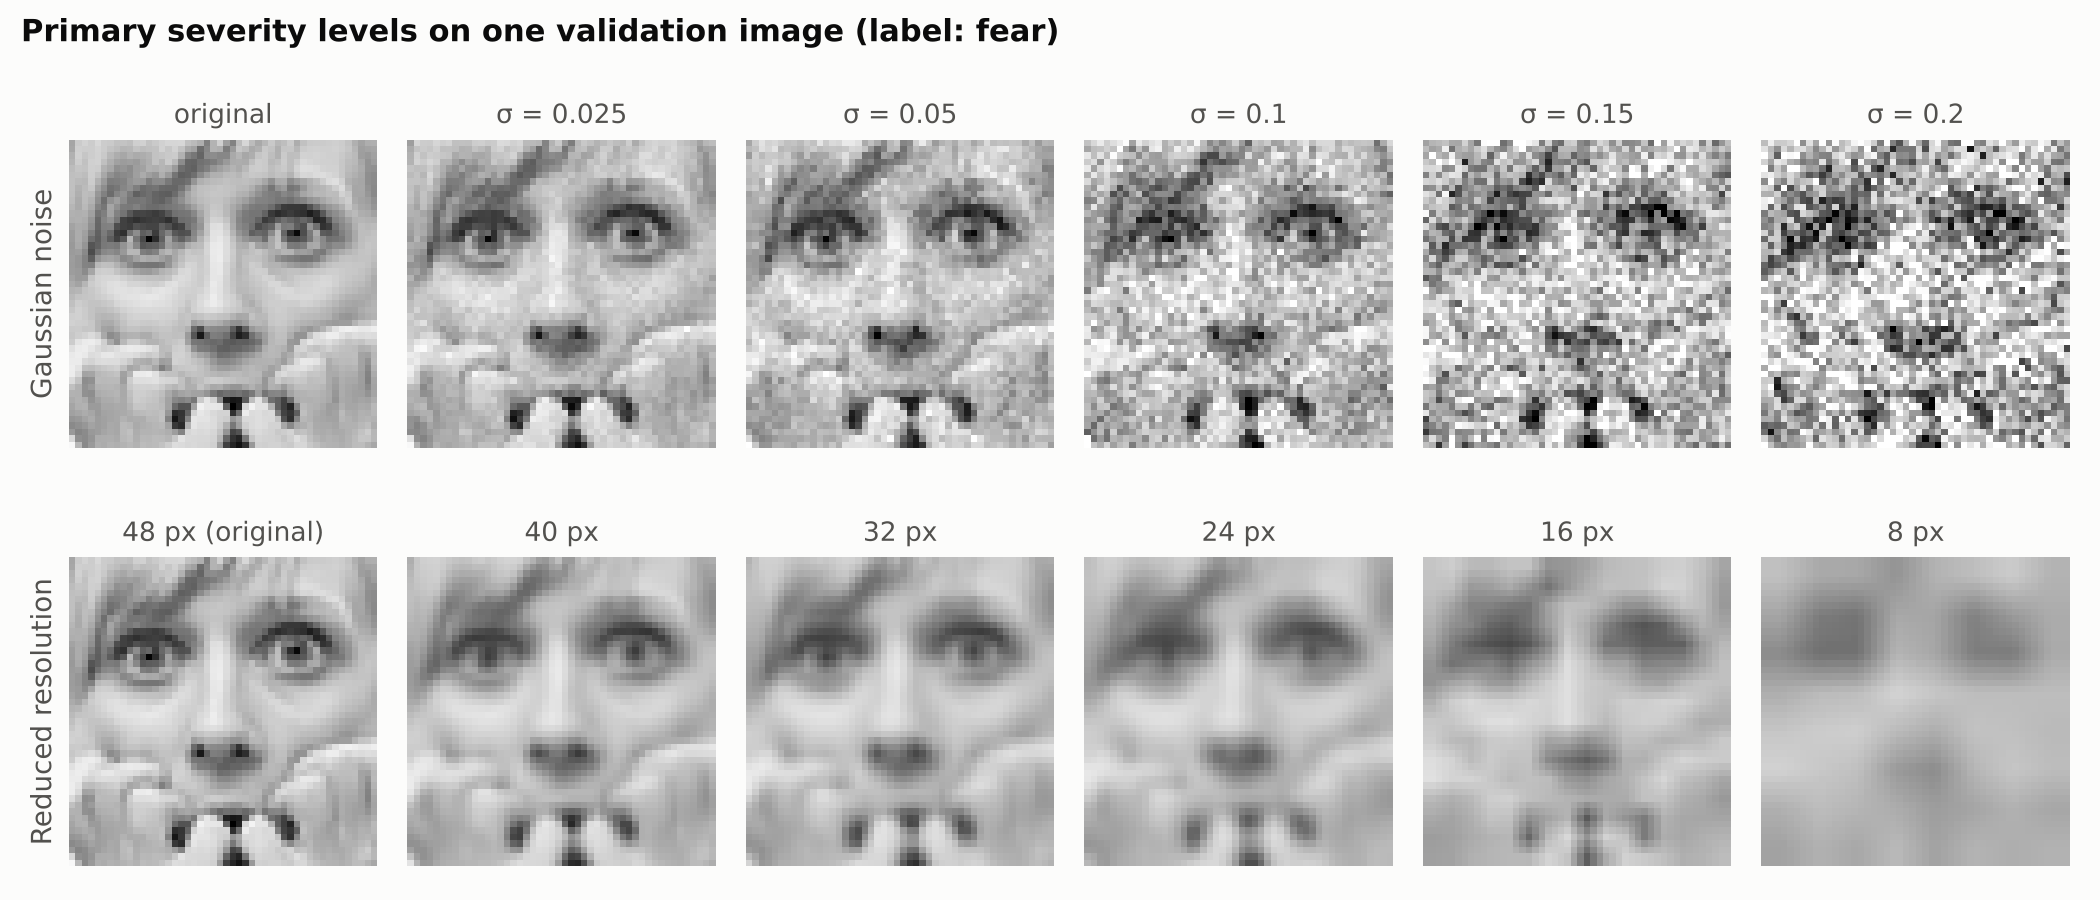
\includegraphics[width=0.8\linewidth]{figures/fig_levels_examples.png}
  \caption{Example validation face across the five primary severity levels for Gaussian noise (top) and reduced
  resolution (bottom). All severity levels were fixed on validation data prior to test evaluation.}
  \label{fig:examples}
\end{figure}

\section{Models and Protocol}
\label{sec:protocol}

\paragraph{Models.}
We compare three architectures that span roughly three orders of magnitude in parameter count. Our \emph{baseline
CNN} is trained from scratch on $48{\times}48$ grayscale images standardized by the training-set mean and standard
deviation; it consists of three $3{\times}3$ convolutional blocks (32, 64, and 128 channels), each followed by ReLU
activation and $2{\times}2$ max pooling, feeding into global average pooling and a linear classifier
(\num{params@cnn} parameters). \emph{ResNet-18}~\cite{he2016resnet} is initialized from torchvision's ImageNet-1K
weights (\num{params@resnet18} parameters), and \emph{ViT-B/16}~\cite{dosovitskiy2021vit} starts from the public
\texttt{google/vit-base-patch16-224} checkpoint, which was pretrained on ImageNet-21k and fine-tuned on ImageNet-1k
(\num{params@vit_b16} parameters). For both pretrained backbones, each grayscale image is replicated across three
channels, resized to $224{\times}224$, and normalized according to the checkpoint's expected statistics; we replace
the classification head with a seven-class linear layer and fine-tune the entire network. Every model is trained with
cross-entropy loss.

\paragraph{Training and model selection.}
The baseline CNN and ResNet-18 are optimized with Adam~\cite{kingma2015adam} using a constant learning rate and batch
size 128, training for up to 150 epochs (early-stopping patience 15) for the CNN and up to 12 epochs (patience 3) for
ResNet-18. For ViT-B/16 we follow a standard fine-tuning setup: AdamW~\cite{loshchilov2019adamw} with weight decay
0.01, batch size 32, and four epochs, using linear warm-up over the first 10\% of steps followed by linear decay. We
intentionally omit all other augmentations (such as random flips or crops) so that Gaussian noise is the sole
variable separating standard and augmented runs.

All model-selection decisions rely on a single validation score,
\begin{equation}
  S \;=\; \tfrac12\,\mathrm{Acc}_{\text{val}}^{\text{original}} \;+\; \tfrac12\,\mathrm{Acc}_{\text{val}}^{\text{noisy}},
  \label{eq:score}
\end{equation}
where the noisy validation accuracy is computed by assigning each validation image to one of the five primary noise
levels. Reduced-resolution images never enter $S$, so test performance on low-resolution faces measures genuine
transfer to an unseen corruption. For each architecture, we use seed~0 alone to (1) choose the learning rate from a
three-point grid under standard training (CNN: $\{3{\times}10^{-4}, 10^{-3}, 3{\times}10^{-3}\}$; ResNet-18:
$\{3{\times}10^{-5}, 10^{-4}, 3{\times}10^{-4}\}$; ViT-B/16: $\{10^{-5}, 2{\times}10^{-5}, 5{\times}10^{-5}\}$),
(2) choose the noise-augmentation parameters at that learning rate, and (3) retain the epoch with the highest $S$
within each training run. Every selected setting was saved and locked before the test set was evaluated
(Appendix~\ref{app:selection}).

\paragraph{Noise augmentation.}
During augmented training, each image is corrupted with probability $p$ by additive Gaussian noise whose standard
deviation is drawn uniformly from $[0,\sigma_{\max}]$, sampled independently for every image and epoch. We select
$(p,\sigma_{\max})$ from $\{0.5, 0.8\}\times\{0.1, 0.2\}$ using the validation score $S$, which picks
$(\num{augp@cnn}, \num{augsigma@cnn})$ for the CNN, $(\num{augp@resnet18}, \num{augsigma@resnet18})$ for ResNet-18,
and $(\num{augp@vit_b16}, \num{augsigma@vit_b16})$ for ViT-B/16.

\paragraph{Final runs and evaluation metrics.}
Each of the six final configurations (three models, trained with and without noise augmentation) is run across three
seeds (0, 1, and 2), and each trained model is evaluated once on the clean and degraded test sets. We report both
overall accuracy and macro-F1 (which gives all seven expressions equal weight), summarized as the mean and sample
standard deviation across the three seeds. Because these three-seed standard deviations capture training variability
rather than confidence intervals, we complement them in Appendix~\ref{app:bootstrap} with bootstrap intervals over
test images holding the trained models fixed. For RQ2, we also track \emph{relative accuracy} (degraded accuracy
divided by the same model's clean accuracy) along with the first severity level where retention drops below 90\%, a
threshold chosen as a practical cutoff for this study. To summarize curves concisely, we report ``noise avg.'' and
``resolution avg.'', defined as the unweighted means across the five primary severity levels of each corruption.

\paragraph{Reference checkpoints.}
\label{sec:ref}
Because Eq.~\eqref{eq:score} places half of its weight on noisy validation accuracy, it tended to pick earlier epochs
during standard training than a clean-only criterion would. To see how much that rule itself moved our baseline
numbers, we trained an additional set of reference runs using the exact same standard-training setup and learning
rates, but picking the checkpoint that maximized original validation accuracy alone (the conventional approach). We
analyze these reference runs separately in Section~\ref{sec:selection-effect} rather than altering the pre-specified
protocol.

\section{Results}
\label{sec:results}

Unless stated otherwise, all figures reported below are test-set averages over three random seeds.

\begin{table}[t]
  \caption{Test accuracy and macro-F1 (\%) on original images and averaged across the five primary severity levels of
  each corruption (mean $\pm$ sample standard deviation over three seeds; best mean per column in bold).}
  \label{tab:main}
  \centering
  \small
  \setlength{\tabcolsep}{4.5pt}
  \resizebox{\linewidth}{!}{\begin{tabular}{llcccccc}
\toprule
 & & \multicolumn{2}{c}{Original images} & \multicolumn{2}{c}{Gaussian noise (avg.)} & \multicolumn{2}{c}{Reduced resolution (avg.)} \\
\cmidrule(lr){3-4}\cmidrule(lr){5-6}\cmidrule(lr){7-8}
Model & Training & Acc. & Macro-F1 & Acc. & Macro-F1 & Acc. & Macro-F1 \\
\midrule
Baseline CNN & standard & 53.2{\scriptsize$\,\pm\,$1.3} & 45.6{\scriptsize$\,\pm\,$2.4} & 37.5{\scriptsize$\,\pm\,$0.4} & 28.8{\scriptsize$\,\pm\,$2.1} & 38.0{\scriptsize$\,\pm\,$0.4} & 28.6{\scriptsize$\,\pm\,$1.7} \\
 & noise aug. & 53.5{\scriptsize$\,\pm\,$0.4} & 45.9{\scriptsize$\,\pm\,$1.1} & 47.5{\scriptsize$\,\pm\,$0.5} & 39.4{\scriptsize$\,\pm\,$0.5} & 39.4{\scriptsize$\,\pm\,$0.3} & 31.2{\scriptsize$\,\pm\,$0.3} \\
\addlinespace
ResNet-18 & standard & 61.2{\scriptsize$\,\pm\,$1.4} & 53.4{\scriptsize$\,\pm\,$5.1} & 37.8{\scriptsize$\,\pm\,$2.5} & 25.3{\scriptsize$\,\pm\,$2.8} & 38.6{\scriptsize$\,\pm\,$0.9} & 27.3{\scriptsize$\,\pm\,$1.5} \\
 & noise aug. & 63.1{\scriptsize$\,\pm\,$1.1} & 57.8{\scriptsize$\,\pm\,$1.1} & 56.7{\scriptsize$\,\pm\,$0.4} & 50.5{\scriptsize$\,\pm\,$1.0} & 47.7{\scriptsize$\,\pm\,$2.3} & 39.3{\scriptsize$\,\pm\,$2.1} \\
\addlinespace
ViT-B/16 & standard & \textbf{69.3}{\scriptsize$\,\pm\,$1.1} & \textbf{65.3}{\scriptsize$\,\pm\,$2.0} & 44.0{\scriptsize$\,\pm\,$0.3} & 37.8{\scriptsize$\,\pm\,$0.6} & 45.8{\scriptsize$\,\pm\,$0.9} & 39.9{\scriptsize$\,\pm\,$0.9} \\
 & noise aug. & 68.5{\scriptsize$\,\pm\,$0.5} & 63.9{\scriptsize$\,\pm\,$0.5} & \textbf{61.9}{\scriptsize$\,\pm\,$0.1} & \textbf{56.3}{\scriptsize$\,\pm\,$0.7} & \textbf{49.8}{\scriptsize$\,\pm\,$0.7} & \textbf{43.2}{\scriptsize$\,\pm\,$0.4} \\
\bottomrule
\end{tabular}
}
\end{table}

\subsection{RQ1: Original Images}
\label{sec:rq1}

On the uncorrupted test images, accuracy climbs steadily with model capacity and pretraining: the baseline CNN
reaches \num{acc@cnn@std@clean}\%, ResNet-18 reaches \num{acc@resnet18@std@clean}\%, and ViT-B/16 reaches
\num{acc@vit_b16@std@clean}\% (Table~\ref{tab:main}). The step-ups between consecutive models
(\num{archdiff@resnet18@cnn@std@clean} and \num{archdiff@vit_b16@resnet18@std@clean} percentage points) are well
outside both the seed-to-seed standard deviations (at most 1.4 points) and test-set sampling uncertainty
(Appendix~\ref{app:bootstrap}).

Macro-F1 sits noticeably below overall accuracy across all three models (\num{macro_f1@cnn@std@clean},
\num{macro_f1@resnet18@std@clean}, and \num{macro_f1@vit_b16@std@clean}), largely because class imbalance hurts
recall on rare or subtle expressions. For instance, the baseline CNN correctly identifies
\num{recall@cnn@std@happy@clean}\% of \emph{happy} faces, yet recovers only \num{recall@cnn@std@disgust@clean}\% of
\emph{disgust} and \num{recall@cnn@std@fear@clean}\% of \emph{fear} examples (Appendix~\ref{app:classes}). ViT-B/16
narrows this gap considerably, lifting \emph{disgust} recall to \num{recall@vit_b16@std@disgust@clean}\%. For rough
context, the dataset's creators estimated human accuracy on unfiltered FER-2013 at
$65\pm5\%$~\cite{goodfellow2013challenges}, though our deduplicated split is not directly comparable.

\subsection{RQ2: Performance under Noise and Reduced Resolution}
\label{sec:rq2}

Under standard training, performance falls off rapidly for all three architectures as image quality drops
(Figure~\ref{fig:degradation}). Every model loses more than 10\% of its clean accuracy by $\sigma=0.05$; under
downsampling, retention dips below 90\% at 32\,px for the CNN and ViT-B/16, and as early as 40\,px for ResNet-18
(Table~\ref{tab:relative}). By $\sigma=0.10$, the CNN, ResNet-18, and ViT-B/16 retain only
\num{rel@cnn@std@n0.1}\%, \num{rel@resnet18@std@n0.1}\%, and \num{rel@vit_b16@std@n0.1}\% of their original accuracy,
respectively. Once degradation becomes severe, the clean-image hierarchy breaks down entirely. At $\sigma=0.20$, all
three models sit within roughly three points of the \num{majority}\% majority-class rate (\num{acc@cnn@std@n0.2}\%
for the CNN, \num{acc@resnet18@std@n0.2}\% for ResNet-18, and \num{acc@vit_b16@std@n0.2}\% for ViT-B/16). At 8\,px,
all three drop below that baseline, and the ordering actually reverses: ViT-B/16, the strongest model on clean
images, ends up the weakest at \num{acc@vit_b16@std@r8}\%, compared with \num{acc@cnn@std@r8}\% for the baseline CNN.

Looking across all five primary levels, the \num{archdiff@resnet18@cnn@std@clean}-point clean advantage that
ResNet-18 holds over the small CNN essentially disappears, shrinking to \num{archdiff@resnet18@cnn@std@navg} points
under noise and \num{archdiff@resnet18@cnn@std@ravg} points under reduced resolution; neither gap can be separated
from zero once test-set sampling error is accounted for (Appendix~\ref{app:bootstrap}). ViT-B/16 holds onto a
meaningful portion of its margin over the CNN (\num{archdiff@vit_b16@cnn@std@navg} points under noise and
\num{archdiff@vit_b16@cnn@std@ravg} under reduced resolution, down from \num{archdiff@vit_b16@cnn@std@clean} on clean
images), yet in relative terms the 94K-parameter CNN retains a higher share of its clean accuracy than either
pretrained model at every single severity level (Table~\ref{tab:relative}). This mirrors what
\citet{hendrycks2019benchmarking} saw on ImageNet-C: scaling up and pretraining raised clean performance
substantially, without making the models more resilient in relative terms.

\begin{figure}[t]
  \centering
  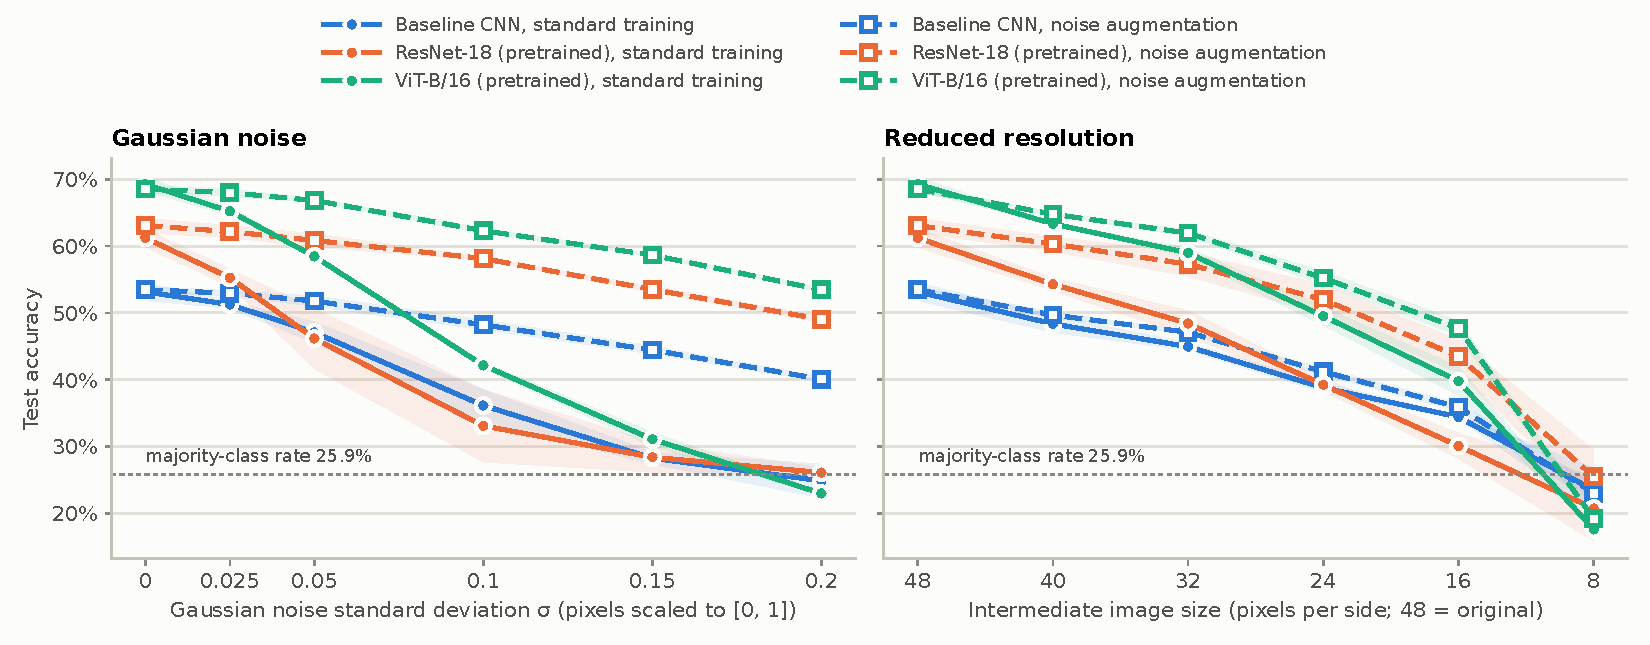
\includegraphics[width=\linewidth]{figures/fig_degradation_acc.pdf}
  \caption{Test accuracy as a function of corruption severity for Gaussian noise (left) and reduced resolution
  (right). Curves show three-seed means, shaded bands show one sample standard deviation, and the dotted line marks
  the majority-class rate.}
  \label{fig:degradation}
\end{figure}

\begin{table}[t]
  \caption{Relative accuracy (\%; degraded accuracy divided by original accuracy, averaged over three seeds) and the
  first tested severity level where retention drops below 90\%.}
  \label{tab:relative}
  \centering
  \small
  \setlength{\tabcolsep}{3.6pt}
  \resizebox{\linewidth}{!}{\begin{tabular}{llcccccccccccc}
\toprule
 & & \multicolumn{6}{c}{Gaussian noise $\sigma$} & \multicolumn{6}{c}{Intermediate size $s$} \\
\cmidrule(lr){3-8}\cmidrule(lr){9-14}
Model & Training & 0.025 & 0.05 & 0.1 & 0.15 & 0.2 & $<$90\% at & 40 & 32 & 24 & 16 & 8 & $<$90\% at \\
\midrule
Baseline CNN & standard & 96 & 89 & 68 & 53 & 47 & $\sigma{=}0.05$ & 91 & 85 & 73 & 65 & 44 & 32\,px \\
 & noise aug. & 99 & 97 & 90 & 83 & 75 & $\sigma{=}0.15$ & 93 & 88 & 77 & 67 & 43 & 32\,px \\
\addlinespace
ResNet-18 & standard & 90 & 76 & 54 & 46 & 43 & $\sigma{=}0.05$ & 89 & 79 & 64 & 49 & 34 & 40\,px \\
 & noise aug. & 99 & 96 & 92 & 85 & 78 & $\sigma{=}0.15$ & 96 & 91 & 82 & 69 & 40 & 24\,px \\
\addlinespace
ViT-B/16 & standard & 94 & 84 & 61 & 45 & 33 & $\sigma{=}0.05$ & 91 & 85 & 72 & 57 & 25 & 32\,px \\
 & noise aug. & 99 & 98 & 91 & 86 & 78 & $\sigma{=}0.15$ & 95 & 90 & 81 & 70 & 28 & 24\,px \\
\bottomrule
\end{tabular}
}
\end{table}

\subsection{RQ3: Effect of Gaussian-Noise Augmentation}
\label{sec:rq3}

\paragraph{Clean images.}
Adding Gaussian noise during training comes with little to no clean-accuracy penalty. Paired by seed against standard
training (Figure~\ref{fig:aug}), noise augmentation produces small shifts on original test accuracy
(\num{delta@cnn@clean} points for the CNN, \num{delta@resnet18@clean} for ResNet-18, and \num{delta@vit_b16@clean}
for ViT-B/16), all modest relative to seed-to-seed variability. Even when measured against the clean-selected
reference checkpoints of Section~\ref{sec:selection-effect}, which provide a slightly stronger clean baseline, the
drop stays under one percentage point for every architecture (\num{augref@cnn@clean}, \num{augref@resnet18@clean},
and \num{augref@vit_b16@clean} points).

\paragraph{Noisy images.}
On noisy test images, the gains are substantial across the board and widen steadily with corruption severity.
Averaged over the five primary noise levels, the accuracy changes are \num{delta@cnn@navg} points for the CNN,
\num{delta@resnet18@navg} for ResNet-18, and \num{delta@vit_b16@navg} for ViT-B/16; at $\sigma=0.20$, they grow to
\num{delta@cnn@n0.2}, \num{delta@resnet18@n0.2}, and \num{delta@vit_b16@n0.2} points. Put differently, noise
augmentation allows all three architectures to hold onto at least 90\% of their clean accuracy through $\sigma=0.10$
(Table~\ref{tab:relative}), whereas standard-trained models already fall below that threshold at $\sigma=0.05$.

\paragraph{Transfer to reduced resolution.}
Because downsampled images never appear during training or model selection, performance under reduced resolution
tests out-of-corruption transfer. Here, the pretrained models and the small CNN diverge sharply: noise augmentation
brings clear low-resolution gains for ResNet-18 (\num{delta@resnet18@ravg} points on average) and ViT-B/16
(\num{delta@vit_b16@ravg} points), compared with only \num{delta@cnn@ravg} points for the baseline CNN. The transfer
benefit peaks at moderate downsampling (at 16\,px, the gains are \num{delta@resnet18@r16}, \num{delta@vit_b16@r16},
and \num{delta@cnn@r16} points) and largely fades out by 8\,px. This pattern aligns well with the frequency analysis
of \citet{yin2019fourier}: training on noisy images discourages a network from leaning on fine high-frequency
textures that downsampling wipes out, but once an image shrinks to $8{\times}8$, too little coarse structure remains
for any model to read the expression reliably. Our experiments do not pinpoint why the small CNN sees almost none of
this transfer. One clear consequence of these gains, however, is that the pretrained networks preserve their
advantage over the baseline CNN across both corruptions once trained with noise (Table~\ref{tab:main}); the breakdown
in model ranking seen in Section~\ref{sec:rq2} is therefore specific to standard training rather than an inherent
weakness of the larger models.

\begin{figure}[t]
  \centering
  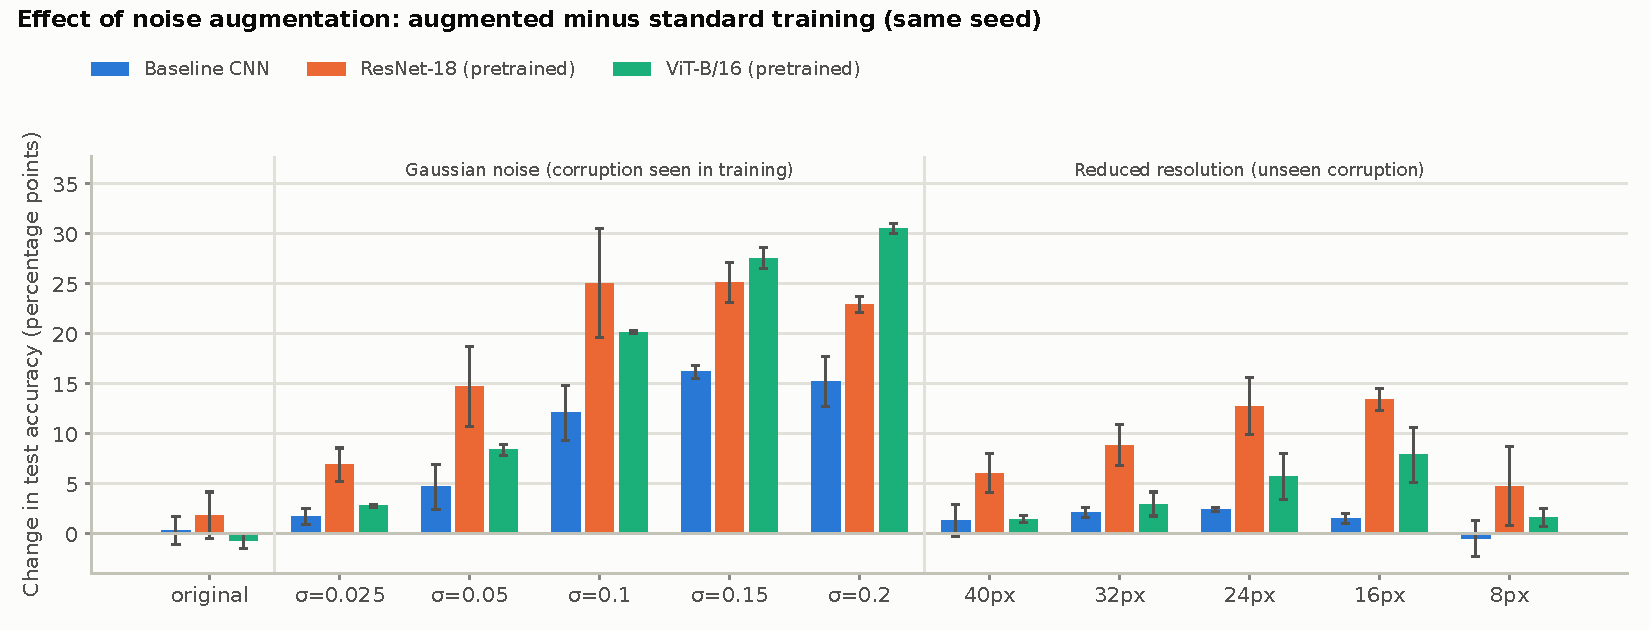
\includegraphics[width=\linewidth]{figures/fig_augmentation_effect.pdf}
  \caption{Effect of Gaussian-noise augmentation on test accuracy (augmented minus standard training, paired by seed;
  mean $\pm$ sample standard deviation). Reduced-resolution images were never used in training or model selection.}
  \label{fig:aug}
\end{figure}

\subsection{Failure Modes and Prediction Collapse}
\label{sec:collapse}

When a classifier's accuracy falls near the majority-class rate, it is worth checking whether its mistakes are spread
across classes or whether it has simply stopped reacting to the input. Figure~\ref{fig:collapse} tracks the fraction
of test images assigned to each model's single most frequently predicted class. On original images, that share sits
between \num{top@vit_b16@std@clean}\% and \num{top@cnn@std@clean}\%, closely matching the \num{majority}\% prevalence
of \emph{happy} in the test split. Under standard training, however, predictions concentrate sharply as degradation
worsens. At $\sigma=0.20$, the CNN, ResNet-18, and ViT-B/16 route \num{top@cnn@std@n0.2}\%,
\num{top@resnet18@std@n0.2}\%, and \num{top@vit_b16@std@n0.2}\% of all test inputs into a single class; at 8\,px,
those shares reach \num{top@cnn@std@r8}\%, \num{top@resnet18@std@r8}\%, and \num{top@vit_b16@std@r8}\%. Because the
fallback class varies across random seeds (often \emph{sad} or \emph{neutral} rather than \emph{happy}), accuracy
can sink below the majority-class baseline. Training with Gaussian noise prevents this collapse under noise, keeping
the top predicted class share within \num{top@resnet18@aug@n0.2}--\num{top@cnn@aug@n0.2}\% at $\sigma=0.20$, though
collapse still returns at 8\,px in line with the limited transfer at extreme downsampling.

Breaking down errors by class shows that \emph{happy} is by far the most resilient expression
(Appendix~\ref{app:classes}). At $\sigma=0.10$, the standard-trained CNN, ResNet-18, and ViT-B/16 still recover
\num{recall@cnn@std@happy@n0.1}\%, \num{recall@resnet18@std@happy@n0.1}\%, and \num{recall@vit_b16@std@happy@n0.1}\%
of \emph{happy} faces. Over the same noisy inputs, recall for \emph{disgust} essentially vanishes (at most
\num{recall@cnn@std@disgust@n0.1}\% across all three models), and \emph{fear} recall drops to
\num{recall@cnn@std@fear@n0.1}\%, \num{recall@resnet18@std@fear@n0.1}\%, and \num{recall@vit_b16@std@fear@n0.1}\%.

\begin{figure}[t]
  \centering
  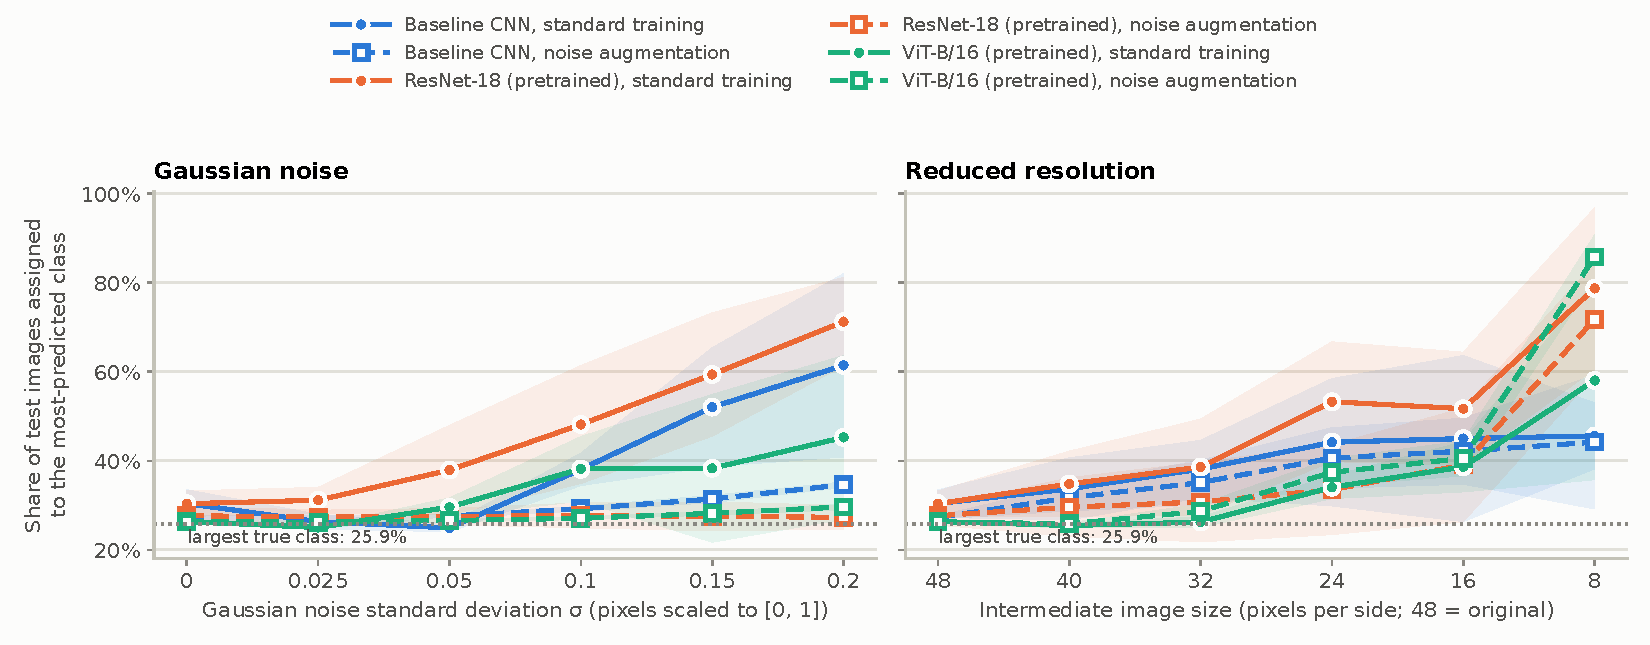
\includegraphics[width=\linewidth]{figures/fig_prediction_collapse.pdf}
  \caption{Share of test images assigned to each model's single most frequently predicted class. Values near the
  dotted majority-class line indicate balanced class usage; high values reflect collapse onto a single prediction.}
  \label{fig:collapse}
\end{figure}

\subsection{Sensitivity to the Checkpoint-Selection Rule}
\label{sec:selection-effect}

When a model is trained only on clean images, its validation accuracy on noisy inputs fluctuates erratically across
epochs and often peaks very early in training (Appendix~\ref{app:curves}). Because our selection score $S$
(Eq.~\ref{eq:score}) weights noisy validation accuracy equally with clean accuracy, it sometimes stopped standard
training well before clean performance plateaued: for ResNet-18, $S$ selected epochs \num{epochs@resnet18@std}, even
though clean validation accuracy kept rising after epoch~1 in two of the three seeds.

To check how much this choice affected our baseline numbers, we repeated standard training using the conventional
rule of picking whichever checkpoint achieved the highest original validation accuracy (Table~\ref{tab:ref},
Appendix~\ref{app:selection}). Under that clean-only rule, both ResNet-18 and the baseline CNN stop at the same epoch
or later. On average, the conventional checkpoints gain \num{refabs@resnet18@clean} points (ResNet-18) and
\num{refabs@cnn@clean} points (CNN) on original images, while giving back \num{refabs@resnet18@navg} and
\num{refabs@cnn@navg} points under noise; the direction of both shifts is consistent across all three seeds for
ResNet-18, though mixed for the CNN. For ViT-B/16, which is fine-tuned for only four epochs, the two selection rules
land at most one epoch apart and differ by less than a point on average (\num{refdelta@vit_b16@clean} on clean images
and \num{refdelta@vit_b16@navg} under noise).

In short, our pre-specified score nudges standard training a few points toward noise robustness at the expense of
clean accuracy on the two smaller networks, while barely touching ViT-B/16. None of the headline findings in
Sections~\ref{sec:rq2} and~\ref{sec:rq3} depend on this choice, however: even with conventional clean-selected
checkpoints, ResNet-18 still fails to outperform the baseline CNN under noise (\num{acc@resnet18@ref@navg}\% vs.\
\num{acc@cnn@ref@navg}\%), ViT-B/16 remains the top model overall, and noise augmentation still adds
\num{augrefabs@cnn@navg} to \num{augrefabs@resnet18@navg} points under noise while costing less than one point on
clean images.

\section{Discussion and Limitations}
\label{sec:discussion}

\paragraph{Practical implications.}
On clean FER-2013 images, the three models line up exactly as capacity and pretraining would suggest. Once images
degrade, however, that clean ranking becomes a poor guide: under standard training, ResNet-18 loses its entire margin
over a CNN with less than one percent as many parameters, and at extreme severity even ViT-B/16 stops responding to
the image content and collapses onto a single class. Adding Gaussian noise during training is an inexpensive fix that
recovers most of the lost performance on noisy inputs at little or no cost to clean accuracy, and for the pretrained
networks it also improves resilience to downsampling despite never seeing low-resolution images during training. For
practitioners deploying expression classifiers on noisy or small face crops, the takeaway is straightforward: test
models under realistic degradation rather than relying on clean accuracy, and include noise augmentation by default.

\paragraph{Limitations.}
Several scope and design choices qualify these conclusions. First, all experiments run on a single dataset of
$48{\times}48$ grayscale crops with known label noise, and those labels reflect annotator judgments of facial
expressions rather than true emotions. We also evaluate only two synthetic corruptions in isolation, whereas real
camera feeds combine sensor noise, motion blur, compression artifacts, lighting shifts, and pose variation at the
same time.

Second, our three models differ simultaneously in architecture, parameter count, and pretraining data, so these
results compare end-to-end modeling choices rather than isolating any single factor. Compute constraints also limited
us to three random seeds per configuration, making the reported standard deviations rough estimates (though the main
effects span many standard deviations). In addition, the selected learning rate fell at the top of our grid for both
pretrained models, and ViT-B/16 was fine-tuned for only four epochs. A post-hoc check one step above the grid changed
the validation score $S$ by less than its seed-to-seed standard deviation (Appendix~\ref{app:selection}), so there is
no sign of a large missed gain, but a single seed cannot rule out a modest one. As shown in
Section~\ref{sec:selection-effect}, the checkpoint-selection rule itself also shifts standard-training results by a
few points for the smaller networks.

Finally, two deliberate protocol constraints affect how the raw numbers should be read. To isolate the effect of
Gaussian noise cleanly, we omitted standard spatial augmentations such as random flips and crops, which leaves our
clean accuracies below the highest figures reported in the literature. Likewise, because degradations are applied
once at the native $48{\times}48$ resolution so that every model is judged on the exact same inputs, upsampling to
$224{\times}224$ introduces spatial correlation into the Gaussian noise seen by ResNet-18 and ViT-B/16.

\paragraph{Future directions.}
The same validation-locked protocol can be extended naturally in several ways: evaluating additional and combined
corruptions (blur, compression, occlusion, and low light), repeating the study with FER+ crowd-sourced label
distributions~\cite{barsoum2016ferplus} to disentangle label ambiguity from model error, and combining noise with
downsampling during training to see whether extreme-resolution collapse at 8\,px can be prevented. Comparing
architectures at matched clean accuracy would also clarify whether any model class provides robustness beyond what
its clean performance alone predicts~\cite{taori2020measuring}.

\section{Conclusion}
\label{sec:conclusion}

Clean test accuracy on FER-2013 gives an overly optimistic picture of how facial-expression classifiers hold up under
noise and low resolution, and it exaggerates the advantage of larger pretrained models under standard training.
Adding Gaussian noise during training offers a simple, low-cost defense that restores much of the lost performance on
noisy inputs and, for pretrained models, transfers partially to unseen resolution loss as well. Going forward,
robustness evaluations are most informative when they report absolute degraded accuracy, relative retention, and the
checkpoint-selection rule side by side.

\begin{ack}
\pending{Statement of contributions and of AI-tool use, as required by the course.}
\end{ack}

{\small
\bibliographystyle{plainnat}
\bibliography{references}
}

\appendix
\raggedbottom

\section{Hyperparameter Selection and Run Details}
\label{app:selection}

Table~\ref{tab:selection} lists the validation selection score $S$ (Eq.~\ref{eq:score}) for every seed-0 tuning run,
with each chosen configuration in bold. For ViT-B/16, the seed-0 final run of each variant reuses the selected tuning
run directly (identical configuration and seed), evaluated once on the test set after settings were locked; the CNN
and ResNet-18 seed-0 runs were retrained.

\begin{table}[H]
  \caption{Validation selection scores $S$ across tuning grids. Left: learning-rate search under standard training.
  Right: noise-augmentation search at the selected learning rate.}
  \label{tab:selection}
  \centering
  \small
  \begin{tabular}{lp{0.36\linewidth}p{0.40\linewidth}}
\toprule
Model & Learning rate: score $S$ & Noise augmentation $(p, \sigma_{\max})$: score $S$ \\
\midrule
Baseline CNN & $3{\times}10^{-4}$: 0.417, \textbf{$1{\times}10^{-3}$: 0.458}, $3{\times}10^{-3}$: 0.446 & (0.5, 0.1): 0.498, \textbf{(0.5, 0.2): 0.515}, (0.8, 0.1): 0.507, (0.8, 0.2): 0.509 \\
ResNet-18 & $3{\times}10^{-5}$: 0.463, $1{\times}10^{-4}$: 0.485, \textbf{$3{\times}10^{-4}$: 0.491} & (0.5, 0.1): 0.581, (0.5, 0.2): 0.595, (0.8, 0.1): 0.580, \textbf{(0.8, 0.2): 0.598} \\
ViT-B/16 & $1{\times}10^{-5}$: 0.532, $2{\times}10^{-5}$: 0.544, \textbf{$5{\times}10^{-5}$: 0.556} & (0.5, 0.1): 0.640, (0.5, 0.2): 0.643, (0.8, 0.1): 0.640, \textbf{(0.8, 0.2): 0.646} \\
\bottomrule
\end{tabular}

\end{table}

Table~\ref{tab:ref} compares the two checkpoint-selection rules for standard training
(Section~\ref{sec:selection-effect}). Because the reference models were trained in separate runs and GPU training is
not bit-for-bit deterministic, any single difference on the scale of the seed standard deviation should be
interpreted with caution.

\begin{table}[H]
  \caption{Standard training with checkpoints chosen by the pre-specified score $S$ versus original validation
  accuracy alone. Test accuracy (\%), mean $\pm$ sample standard deviation over three seeds; difference rows are
  paired by seed (mean $\pm$ standard deviation of the three differences).}
  \label{tab:ref}
  \centering
  \small
  \begin{tabular}{llcccc}
\toprule
Model & Checkpoint rule & Epochs & Original & Noise avg. & Resolution avg. \\
\midrule
Baseline CNN & score $S$ & 28, 22, 32 & 53.2{\scriptsize$\,\pm\,$1.3} & 37.5{\scriptsize$\,\pm\,$0.4} & 38.0{\scriptsize$\,\pm\,$0.4} \\
 & original only & 32, 60, 58 & 53.9{\scriptsize$\,\pm\,$0.5} & 34.4{\scriptsize$\,\pm\,$3.6} & 38.7{\scriptsize$\,\pm\,$2.1} \\
 & \emph{difference} & & +0.8{\scriptsize$\,\pm\,$1.0} & $-$3.1{\scriptsize$\,\pm\,$3.8} & +0.7{\scriptsize$\,\pm\,$1.9} \\
\addlinespace
ResNet-18 & score $S$ & 6, 1, 1 & 61.2{\scriptsize$\,\pm\,$1.4} & 37.8{\scriptsize$\,\pm\,$2.5} & 38.6{\scriptsize$\,\pm\,$0.9} \\
 & original only & 6, 2, 4 & 63.7{\scriptsize$\,\pm\,$0.3} & 33.7{\scriptsize$\,\pm\,$2.8} & 39.7{\scriptsize$\,\pm\,$1.2} \\
 & \emph{difference} & & +2.5{\scriptsize$\,\pm\,$1.6} & $-$4.1{\scriptsize$\,\pm\,$4.3} & +1.1{\scriptsize$\,\pm\,$1.6} \\
\addlinespace
ViT-B/16 & score $S$ & 3, 2, 4 & 69.3{\scriptsize$\,\pm\,$1.1} & 44.0{\scriptsize$\,\pm\,$0.3} & 45.8{\scriptsize$\,\pm\,$0.9} \\
 & original only & 4, 3, 4 & 69.5{\scriptsize$\,\pm\,$0.4} & 43.2{\scriptsize$\,\pm\,$0.3} & 45.7{\scriptsize$\,\pm\,$0.4} \\
 & \emph{difference} & & +0.2{\scriptsize$\,\pm\,$0.7} & $-$0.8{\scriptsize$\,\pm\,$0.5} & $-$0.2{\scriptsize$\,\pm\,$0.6} \\
\bottomrule
\end{tabular}

\end{table}

\paragraph{Post-hoc learning-rate check.}
The chosen learning rate fell at the upper edge of our grid for both pretrained models. After completing the main
protocol, we ran standard training once more at one step higher (seed~0, validation images only; these runs played no
part in selection or test evaluation). ResNet-18 at \num{lrcheck@resnet18@lr} reached
$S=\num{lrcheck@resnet18@score}$ (\num{lrcheck@resnet18@clean}\% original, \num{lrcheck@resnet18@noisy}\% noisy),
compared with \num{lrcheck@resnet18@selscore} at the selected \num{lr@resnet18}. ViT-B/16 at
\num{lrcheck@vit_b16@lr} reached $S=\num{lrcheck@vit_b16@score}$ (\num{lrcheck@vit_b16@clean}\% original,
\num{lrcheck@vit_b16@noisy}\% noisy), compared with \num{lrcheck@vit_b16@selscore} at the selected \num{lr@vit_b16}.
For comparison, the three-seed standard deviation of $S$ at the chosen learning rates is \num{scoresd@resnet18} for
ResNet-18 and \num{scoresd@vit_b16} for ViT-B/16. A single seed cannot rule out a slight improvement from a larger
step size, but there is no indication of a meaningful gain.

\paragraph{Compute and software.}
All experiments ran on a single NVIDIA T4 GPU with automatic mixed precision. The tuning runs, all \num{nfinal}
protocol runs, and the CNN and ResNet-18 reference runs were executed on Google Colab with PyTorch~2.14. The ViT-B/16
reference runs and the post-hoc learning-rate check were executed on Kaggle with PyTorch~2.11 using the exact same
code, deduplicated dataset, and locked settings; consequently, the ViT-B/16 rows of Table~\ref{tab:ref} and the
learning-rate check compare runs across two PyTorch versions. Training the \num{nfinal} protocol runs and \num{nref}
reference runs required roughly \num{gpuhours@final} GPU-hours in total, or about 20 minutes per ViT-B/16 run,
excluding tuning and test evaluation.

\section{Validation Curves}
\label{app:curves}

\begin{figure}[H]
  \centering
  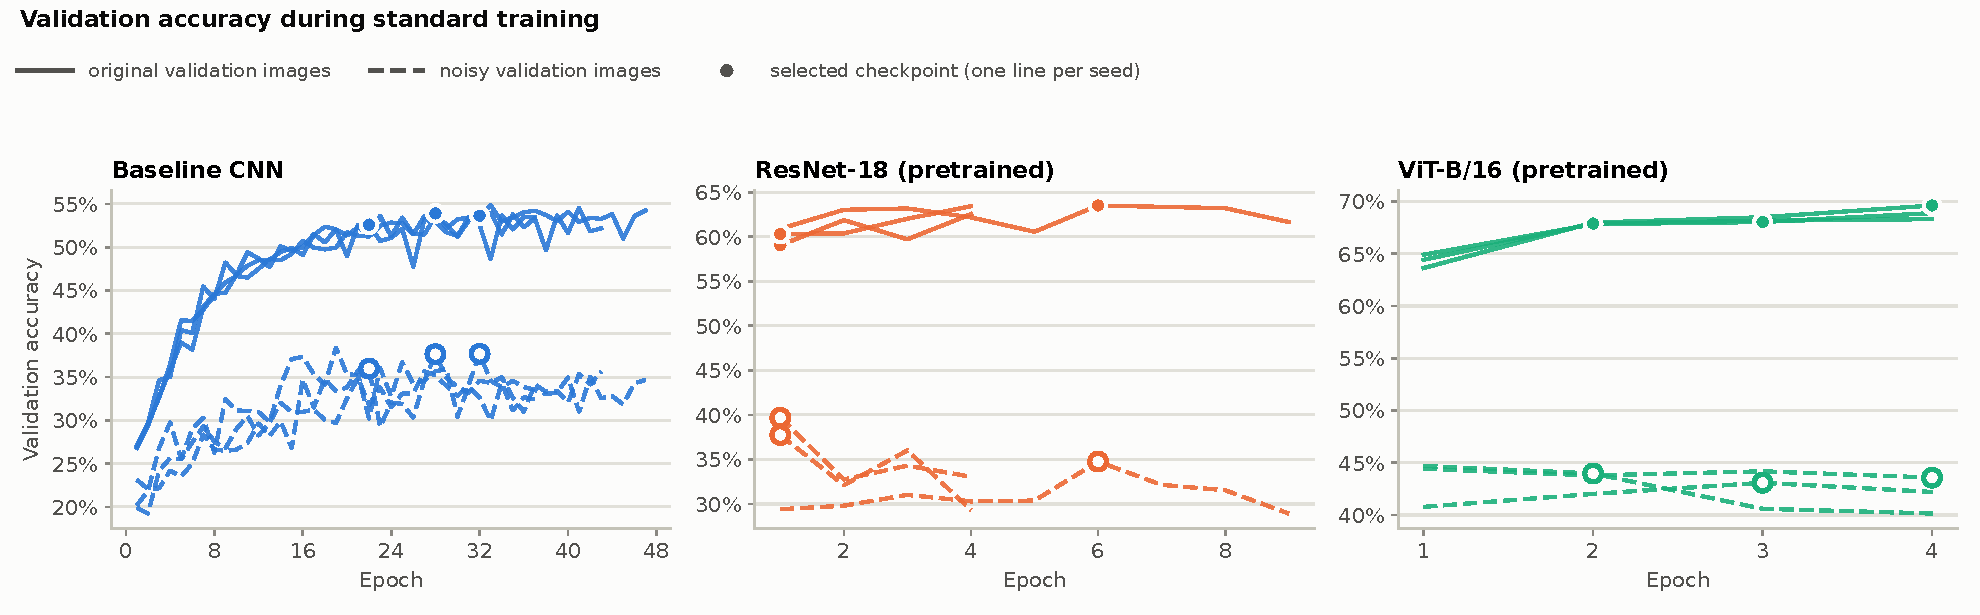
\includegraphics[width=\linewidth]{figures/fig_learning_curves.pdf}
  \caption{Validation accuracy per epoch under standard training on original (solid) and noisy (dashed) validation
  images, with one curve per seed. Markers indicate the checkpoint selected by the pre-specified score $S$.}
  \label{fig:curves}
\end{figure}

\section{Accuracy Across All Severity Levels}
\label{app:levels}

\begin{table}[H]
  \caption{Test accuracy (\%) under Gaussian noise, including the extended levels $\sigma\ge0.3$.}
  \centering
  \scriptsize
  \setlength{\tabcolsep}{3pt}
  \resizebox{\linewidth}{!}{\begin{tabular}{llccccccccc}
\toprule
 & & & \multicolumn{8}{c}{Noise standard deviation $\sigma$} \\
\cmidrule(lr){4-11}
Model & Training & Original & 0.025 & 0.05 & 0.1 & 0.15 & 0.2 & 0.3 & 0.4 & 0.5 \\
\midrule
Baseline CNN & standard & 53.2{\scriptsize$\,\pm\,$1.3} & 51.3{\scriptsize$\,\pm\,$0.5} & 47.1{\scriptsize$\,\pm\,$1.5} & 36.1{\scriptsize$\,\pm\,$2.4} & 28.3{\scriptsize$\,\pm\,$0.9} & 24.9{\scriptsize$\,\pm\,$2.5} & 23.5{\scriptsize$\,\pm\,$3.2} & 22.5{\scriptsize$\,\pm\,$3.3} & 22.1{\scriptsize$\,\pm\,$3.8} \\
 & noise aug. & 53.5{\scriptsize$\,\pm\,$0.4} & 52.9{\scriptsize$\,\pm\,$0.4} & 51.8{\scriptsize$\,\pm\,$0.8} & 48.2{\scriptsize$\,\pm\,$0.7} & 44.4{\scriptsize$\,\pm\,$0.6} & 40.1{\scriptsize$\,\pm\,$0.4} & 33.3{\scriptsize$\,\pm\,$0.2} & 28.6{\scriptsize$\,\pm\,$0.6} & 26.9{\scriptsize$\,\pm\,$0.9} \\
\addlinespace
ResNet-18 & standard & 61.2{\scriptsize$\,\pm\,$1.4} & 55.3{\scriptsize$\,\pm\,$1.2} & 46.2{\scriptsize$\,\pm\,$4.5} & 33.1{\scriptsize$\,\pm\,$5.4} & 28.4{\scriptsize$\,\pm\,$2.2} & 26.1{\scriptsize$\,\pm\,$0.7} & 23.4{\scriptsize$\,\pm\,$3.9} & 22.9{\scriptsize$\,\pm\,$4.5} & 21.8{\scriptsize$\,\pm\,$4.2} \\
 & noise aug. & 63.1{\scriptsize$\,\pm\,$1.1} & 62.2{\scriptsize$\,\pm\,$0.9} & 60.8{\scriptsize$\,\pm\,$1.0} & 58.1{\scriptsize$\,\pm\,$0.3} & 53.5{\scriptsize$\,\pm\,$0.4} & 49.0{\scriptsize$\,\pm\,$0.5} & 40.4{\scriptsize$\,\pm\,$0.5} & 33.3{\scriptsize$\,\pm\,$0.7} & 27.6{\scriptsize$\,\pm\,$1.2} \\
\addlinespace
ViT-B/16 & standard & 69.3{\scriptsize$\,\pm\,$1.1} & 65.2{\scriptsize$\,\pm\,$0.6} & 58.5{\scriptsize$\,\pm\,$0.2} & 42.1{\scriptsize$\,\pm\,$0.4} & 31.1{\scriptsize$\,\pm\,$1.1} & 23.0{\scriptsize$\,\pm\,$0.3} & 18.2{\scriptsize$\,\pm\,$0.6} & 16.6{\scriptsize$\,\pm\,$1.1} & 15.7{\scriptsize$\,\pm\,$0.9} \\
 & noise aug. & 68.5{\scriptsize$\,\pm\,$0.5} & 68.0{\scriptsize$\,\pm\,$0.6} & 66.8{\scriptsize$\,\pm\,$0.3} & 62.3{\scriptsize$\,\pm\,$0.4} & 58.6{\scriptsize$\,\pm\,$0.2} & 53.5{\scriptsize$\,\pm\,$0.3} & 45.2{\scriptsize$\,\pm\,$0.6} & 38.9{\scriptsize$\,\pm\,$0.6} & 34.0{\scriptsize$\,\pm\,$0.6} \\
\bottomrule
\end{tabular}
}
\end{table}

\begin{table}[H]
  \caption{Test accuracy (\%) under reduced resolution, including the extended level $s=4$.}
  \centering
  \scriptsize
  \setlength{\tabcolsep}{3pt}
  \resizebox{\linewidth}{!}{\begin{tabular}{llccccccc}
\toprule
 & & & \multicolumn{6}{c}{Intermediate size $s$ (pixels)} \\
\cmidrule(lr){4-9}
Model & Training & Original & 40 & 32 & 24 & 16 & 8 & 4 \\
\midrule
Baseline CNN & standard & 53.2{\scriptsize$\,\pm\,$1.3} & 48.4{\scriptsize$\,\pm\,$1.3} & 45.0{\scriptsize$\,\pm\,$0.6} & 38.8{\scriptsize$\,\pm\,$0.7} & 34.4{\scriptsize$\,\pm\,$0.3} & 23.5{\scriptsize$\,\pm\,$3.3} & 14.7{\scriptsize$\,\pm\,$2.8} \\
 & noise aug. & 53.5{\scriptsize$\,\pm\,$0.4} & 49.7{\scriptsize$\,\pm\,$0.4} & 47.1{\scriptsize$\,\pm\,$0.2} & 41.2{\scriptsize$\,\pm\,$0.5} & 35.9{\scriptsize$\,\pm\,$0.6} & 23.0{\scriptsize$\,\pm\,$1.5} & 16.3{\scriptsize$\,\pm\,$1.2} \\
\addlinespace
ResNet-18 & standard & 61.2{\scriptsize$\,\pm\,$1.4} & 54.3{\scriptsize$\,\pm\,$1.0} & 48.4{\scriptsize$\,\pm\,$1.9} & 39.2{\scriptsize$\,\pm\,$0.9} & 30.1{\scriptsize$\,\pm\,$1.9} & 20.7{\scriptsize$\,\pm\,$4.8} & 19.1{\scriptsize$\,\pm\,$3.1} \\
 & noise aug. & 63.1{\scriptsize$\,\pm\,$1.1} & 60.3{\scriptsize$\,\pm\,$1.1} & 57.3{\scriptsize$\,\pm\,$1.8} & 52.0{\scriptsize$\,\pm\,$2.2} & 43.5{\scriptsize$\,\pm\,$2.4} & 25.5{\scriptsize$\,\pm\,$4.0} & 23.7{\scriptsize$\,\pm\,$4.0} \\
\addlinespace
ViT-B/16 & standard & 69.3{\scriptsize$\,\pm\,$1.1} & 63.3{\scriptsize$\,\pm\,$0.1} & 59.0{\scriptsize$\,\pm\,$0.7} & 49.5{\scriptsize$\,\pm\,$1.4} & 39.8{\scriptsize$\,\pm\,$2.1} & 17.6{\scriptsize$\,\pm\,$0.4} & 17.2{\scriptsize$\,\pm\,$0.7} \\
 & noise aug. & 68.5{\scriptsize$\,\pm\,$0.5} & 64.8{\scriptsize$\,\pm\,$0.3} & 61.9{\scriptsize$\,\pm\,$0.5} & 55.2{\scriptsize$\,\pm\,$1.0} & 47.7{\scriptsize$\,\pm\,$1.1} & 19.2{\scriptsize$\,\pm\,$0.7} & 17.5{\scriptsize$\,\pm\,$0.3} \\
\bottomrule
\end{tabular}
}
\end{table}

\begin{table}[H]
  \caption{Change in test accuracy from Gaussian-noise augmentation at every primary level (percentage points;
  augmented minus standard training, paired by seed).}
  \centering
  \scriptsize
  \setlength{\tabcolsep}{2.5pt}
  \resizebox{\linewidth}{!}{\begin{tabular}{lccccccccccc}
\toprule
 & & \multicolumn{5}{c}{Gaussian noise $\sigma$ (seen in training)} & \multicolumn{5}{c}{Intermediate size $s$ (never seen)} \\
\cmidrule(lr){3-7}\cmidrule(lr){8-12}
Model & Original & 0.025 & 0.05 & 0.1 & 0.15 & 0.2 & 40 & 32 & 24 & 16 & 8 \\
\midrule
Baseline CNN & +0.3{\scriptsize$\,\pm\,$1.4} & +1.7{\scriptsize$\,\pm\,$0.8} & +4.7{\scriptsize$\,\pm\,$2.3} & +12.1{\scriptsize$\,\pm\,$2.7} & +16.2{\scriptsize$\,\pm\,$0.7} & +15.2{\scriptsize$\,\pm\,$2.5} & +1.3{\scriptsize$\,\pm\,$1.6} & +2.1{\scriptsize$\,\pm\,$0.5} & +2.4{\scriptsize$\,\pm\,$0.2} & +1.5{\scriptsize$\,\pm\,$0.5} & $-$0.5{\scriptsize$\,\pm\,$1.8} \\
ResNet-18 & +1.8{\scriptsize$\,\pm\,$2.3} & +6.9{\scriptsize$\,\pm\,$1.7} & +14.7{\scriptsize$\,\pm\,$4.0} & +25.0{\scriptsize$\,\pm\,$5.4} & +25.1{\scriptsize$\,\pm\,$2.0} & +22.9{\scriptsize$\,\pm\,$0.8} & +6.0{\scriptsize$\,\pm\,$2.0} & +8.9{\scriptsize$\,\pm\,$2.1} & +12.7{\scriptsize$\,\pm\,$2.9} & +13.4{\scriptsize$\,\pm\,$1.1} & +4.8{\scriptsize$\,\pm\,$3.9} \\
ViT-B/16 & $-$0.7{\scriptsize$\,\pm\,$0.8} & +2.8{\scriptsize$\,\pm\,$0.2} & +8.4{\scriptsize$\,\pm\,$0.5} & +20.2{\scriptsize$\,\pm\,$0.2} & +27.6{\scriptsize$\,\pm\,$1.0} & +30.5{\scriptsize$\,\pm\,$0.5} & +1.4{\scriptsize$\,\pm\,$0.4} & +3.0{\scriptsize$\,\pm\,$1.2} & +5.7{\scriptsize$\,\pm\,$2.3} & +7.9{\scriptsize$\,\pm\,$2.7} & +1.6{\scriptsize$\,\pm\,$0.9} \\
\bottomrule
\end{tabular}
}
\end{table}

\section{Test-Set Sampling Uncertainty}
\label{app:bootstrap}

Table~\ref{tab:bootstrap} reports 95\% percentile-bootstrap intervals obtained by resampling the \num{ntest} test
images 5{,}000 times while keeping the trained models fixed. These intervals isolate test-set sampling uncertainty
and complement the seed-to-seed standard deviations reported in the main text.

\begin{table}[H]
  \caption{Seed-averaged test accuracy and pairwise differences with 95\% bootstrap intervals over test images.
  $^{*}$: interval excludes zero. ``clean-sel.'': standard training with checkpoints selected on original validation
  accuracy only.}
  \label{tab:bootstrap}
  \centering
  \small
  \begin{tabular}{lccc}
\toprule
 & Original & Noise avg. & Resolution avg. \\
\midrule
\multicolumn{4}{l}{\emph{Seed-averaged accuracy (\%)}} \\
Baseline CNN, standard & 53.2{\scriptsize\,[51.7, 54.6]} & 37.5{\scriptsize\,[36.5, 38.5]} & 38.0{\scriptsize\,[36.9, 39.1]} \\
Baseline CNN, noise aug. & 53.5{\scriptsize\,[52.0, 54.9]} & 47.5{\scriptsize\,[46.3, 48.8]} & 39.4{\scriptsize\,[38.3, 40.6]} \\
Baseline CNN, clean-sel. & 53.9{\scriptsize\,[52.5, 55.4]} & 34.4{\scriptsize\,[33.5, 35.2]} & 38.7{\scriptsize\,[37.6, 39.8]} \\
ResNet-18, standard & 61.2{\scriptsize\,[59.9, 62.6]} & 37.8{\scriptsize\,[36.8, 38.8]} & 38.6{\scriptsize\,[37.5, 39.5]} \\
ResNet-18, noise aug. & 63.1{\scriptsize\,[61.7, 64.5]} & 56.7{\scriptsize\,[55.5, 58.0]} & 47.7{\scriptsize\,[46.6, 48.9]} \\
ResNet-18, clean-sel. & 63.7{\scriptsize\,[62.4, 65.1]} & 33.7{\scriptsize\,[32.8, 34.6]} & 39.7{\scriptsize\,[38.8, 40.6]} \\
ViT-B/16, standard & 69.3{\scriptsize\,[67.8, 70.7]} & 44.0{\scriptsize\,[43.0, 44.9]} & 45.8{\scriptsize\,[44.8, 46.9]} \\
ViT-B/16, noise aug. & 68.5{\scriptsize\,[67.0, 70.0]} & 61.9{\scriptsize\,[60.6, 63.2]} & 49.8{\scriptsize\,[48.6, 51.0]} \\
ViT-B/16, clean-sel. & 69.5{\scriptsize\,[68.0, 70.9]} & 43.2{\scriptsize\,[42.3, 44.2]} & 45.7{\scriptsize\,[44.7, 46.7]} \\
\addlinespace
\multicolumn{4}{l}{\emph{Noise augmentation minus standard training (points)}} \\
Baseline CNN & +0.3{\scriptsize\,[$-$0.6, +1.3]} & +10.0{\scriptsize\,[+9.1, +10.8]}$^{*}$ & +1.4{\scriptsize\,[+0.7, +2.1]}$^{*}$ \\
ResNet-18 & +1.8{\scriptsize\,[+0.8, +2.8]}$^{*}$ & +18.9{\scriptsize\,[+17.9, +20.0]}$^{*}$ & +9.2{\scriptsize\,[+8.4, +9.9]}$^{*}$ \\
ViT-B/16 & $-$0.7{\scriptsize\,[$-$1.5, +0.0]} & +17.9{\scriptsize\,[+16.9, +18.8]}$^{*}$ & +3.9{\scriptsize\,[+3.3, +4.5]}$^{*}$ \\
\addlinespace
\multicolumn{4}{l}{\emph{Clean-selected minus score-selected checkpoint (points)}} \\
Baseline CNN & +0.8{\scriptsize\,[$-$0.1, +1.6]} & $-$3.1{\scriptsize\,[$-$3.8, $-$2.5]}$^{*}$ & +0.7{\scriptsize\,[+0.1, +1.2]}$^{*}$ \\
ResNet-18 & +2.5{\scriptsize\,[+1.5, +3.5]}$^{*}$ & $-$4.1{\scriptsize\,[$-$5.0, $-$3.3]}$^{*}$ & +1.1{\scriptsize\,[+0.5, +1.8]}$^{*}$ \\
ViT-B/16 & +0.2{\scriptsize\,[$-$0.4, +0.8]} & $-$0.8{\scriptsize\,[$-$1.1, $-$0.4]}$^{*}$ & $-$0.2{\scriptsize\,[$-$0.6, +0.2]} \\
\addlinespace
\multicolumn{4}{l}{\emph{Between architectures, standard training (points)}} \\
ResNet-18 $-$ Baseline CNN & +8.1{\scriptsize\,[+6.9, +9.3]}$^{*}$ & +0.3{\scriptsize\,[$-$0.7, +1.3]} & +0.6{\scriptsize\,[$-$0.2, +1.3]} \\
ViT-B/16 $-$ Baseline CNN & +16.1{\scriptsize\,[+14.7, +17.5]}$^{*}$ & +6.5{\scriptsize\,[+5.5, +7.5]}$^{*}$ & +7.8{\scriptsize\,[+6.8, +8.9]}$^{*}$ \\
ViT-B/16 $-$ ResNet-18 & +8.0{\scriptsize\,[+7.0, +9.1]}$^{*}$ & +6.2{\scriptsize\,[+5.2, +7.1]}$^{*}$ & +7.3{\scriptsize\,[+6.4, +8.2]}$^{*}$ \\
\addlinespace
\multicolumn{4}{l}{\emph{Between architectures, noise augmentation (points)}} \\
ResNet-18 $-$ Baseline CNN & +9.6{\scriptsize\,[+8.4, +10.8]}$^{*}$ & +9.2{\scriptsize\,[+8.4, +10.1]}$^{*}$ & +8.3{\scriptsize\,[+7.5, +9.2]}$^{*}$ \\
ViT-B/16 $-$ Baseline CNN & +15.1{\scriptsize\,[+13.7, +16.5]}$^{*}$ & +14.4{\scriptsize\,[+13.3, +15.4]}$^{*}$ & +10.4{\scriptsize\,[+9.3, +11.4]}$^{*}$ \\
ViT-B/16 $-$ ResNet-18 & +5.5{\scriptsize\,[+4.4, +6.5]}$^{*}$ & +5.1{\scriptsize\,[+4.3, +5.9]}$^{*}$ & +2.1{\scriptsize\,[+1.2, +2.9]}$^{*}$ \\
\bottomrule
\end{tabular}

\end{table}

\section{Per-Class Results}
\label{app:classes}

\begin{table}[H]
  \caption{Per-class recall (\%) on original test images, averaged over three seeds.}
  \centering
  \small
  \begin{tabular}{llccccccc}
\toprule
Model & Training & Angry & Disgust & Fear & Happy & Sad & Surprise & Neutral \\
\midrule
Baseline CNN & standard & 41.0 & 10.5 & 31.0 & 81.5 & 42.4 & 61.2 & 49.2 \\
 & noise aug. & 34.2 & 9.6 & 30.3 & 77.8 & 50.0 & 58.9 & 55.7 \\
\addlinespace
ResNet-18 & standard & 52.7 & 18.4 & 39.9 & 90.9 & 48.9 & 64.7 & 55.6 \\
 & noise aug. & 51.3 & 29.8 & 37.3 & 86.6 & 52.8 & 68.4 & 68.7 \\
\addlinespace
ViT-B/16 & standard & 62.7 & 53.5 & 47.6 & 91.1 & 56.3 & 76.9 & 70.5 \\
 & noise aug. & 60.3 & 40.4 & 46.9 & 91.0 & 57.2 & 72.8 & 70.9 \\
\bottomrule
\end{tabular}

\end{table}

\begin{figure}[H]
  \centering
  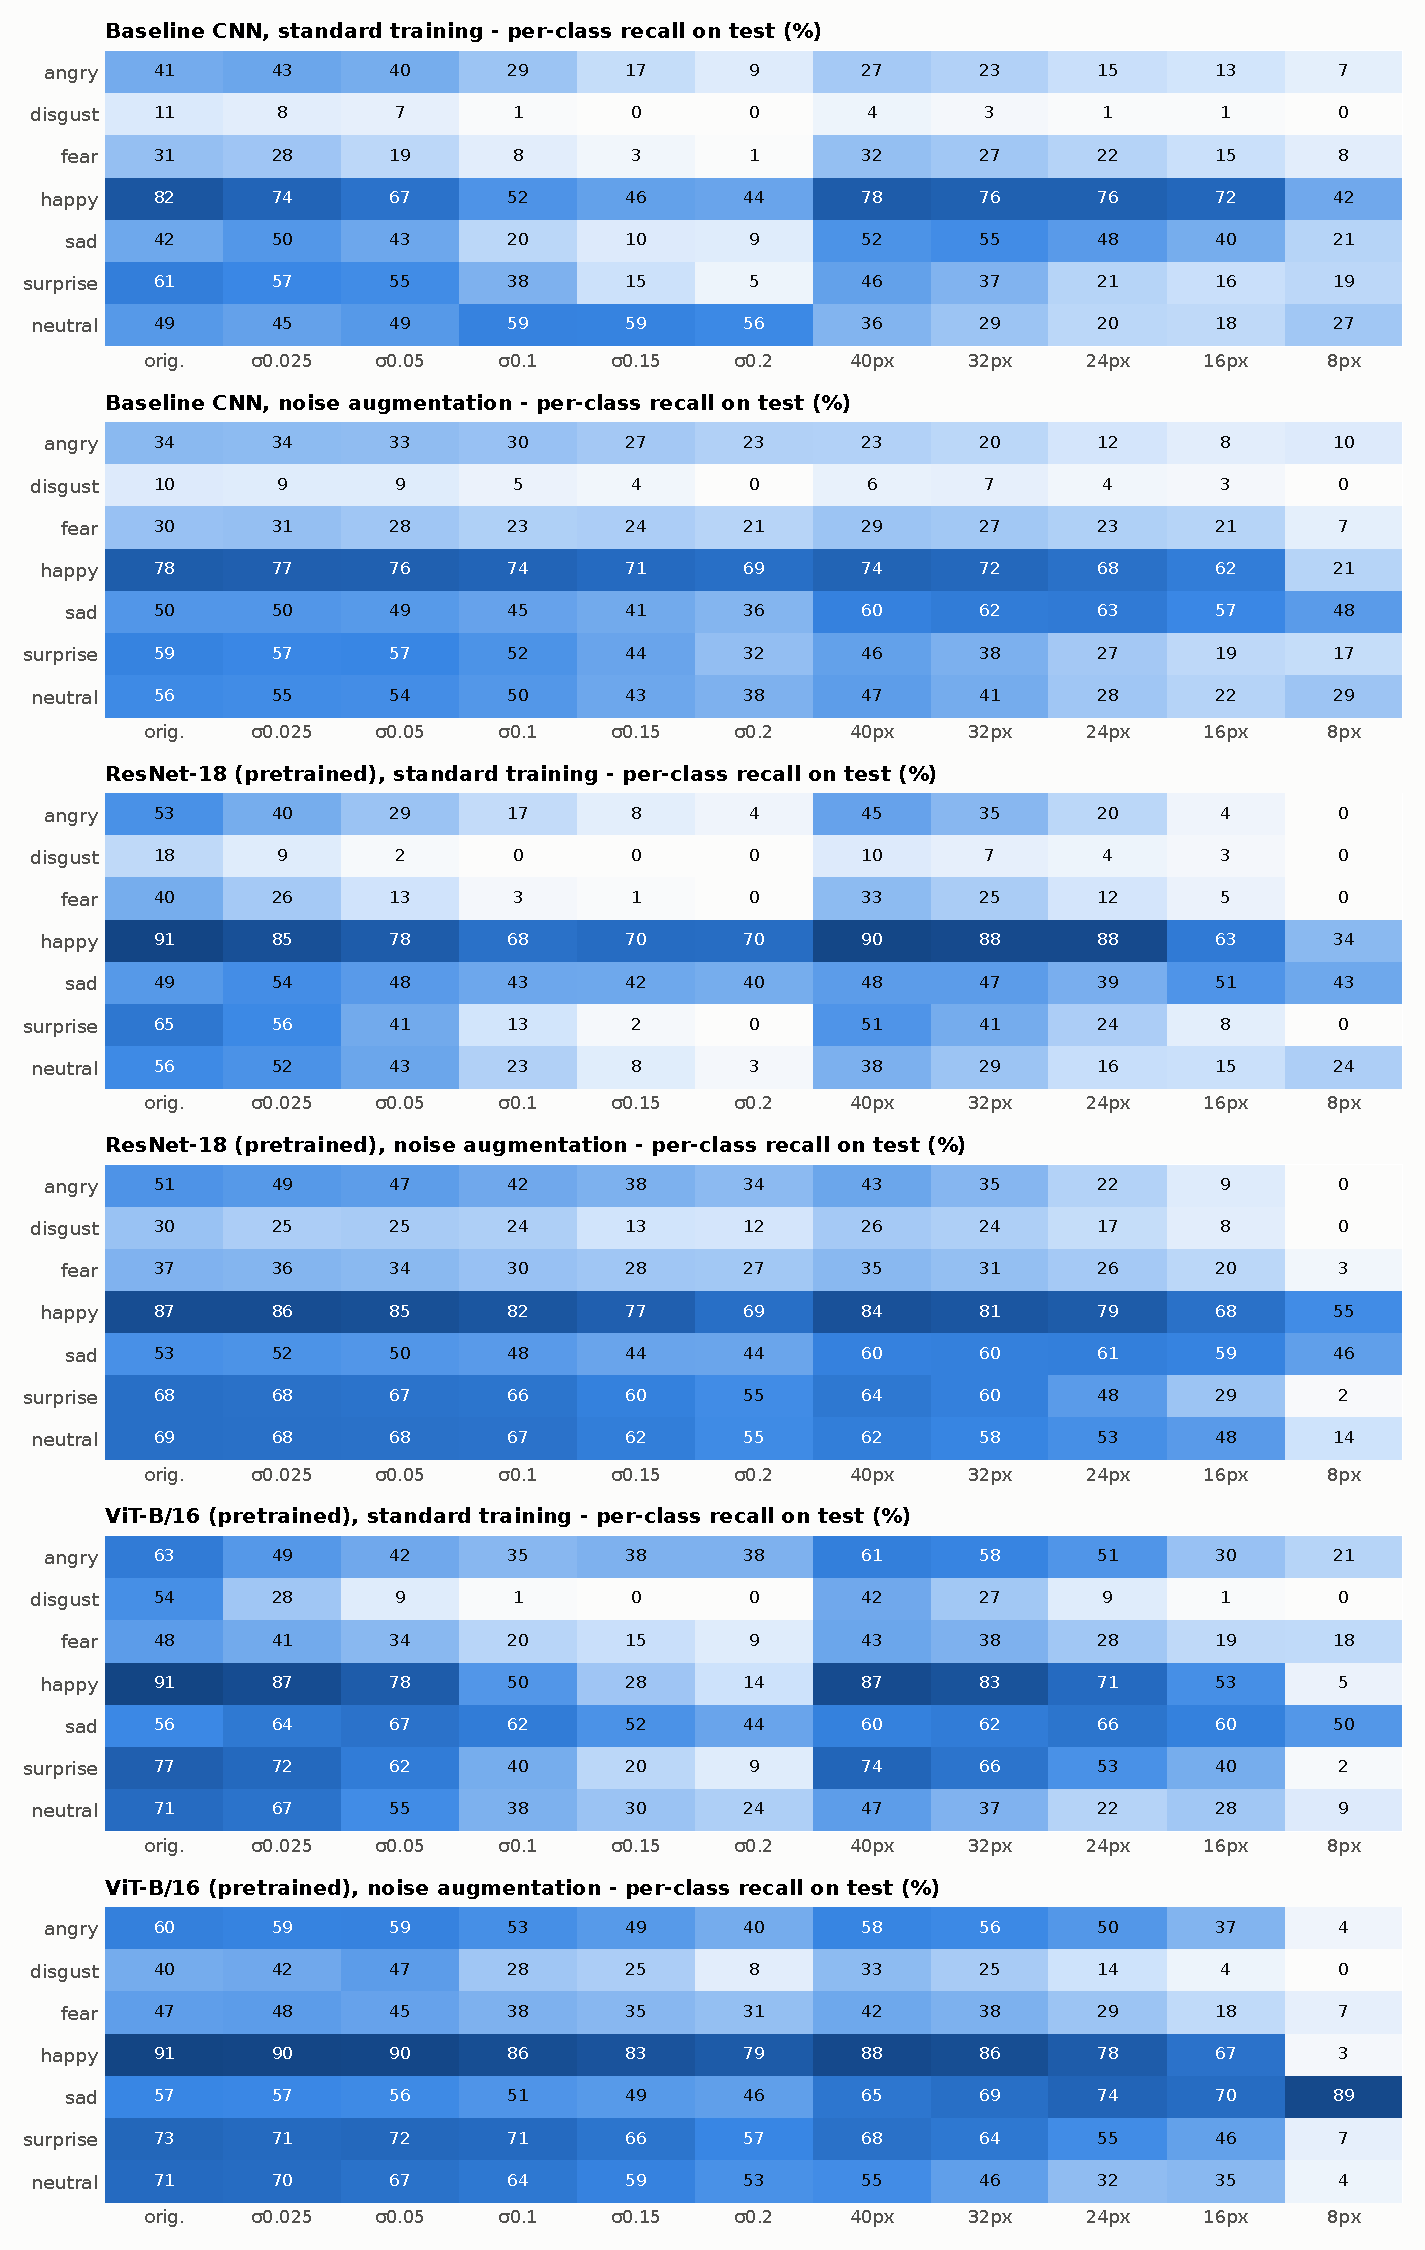
\includegraphics[width=0.96\linewidth]{figures/fig_per_class_recall.pdf}
  \caption{Per-class recall across all primary severity levels.}
\end{figure}

\end{document}
